\documentclass[twoside,11pt]{article}
\usepackage{jair,theapa, rawfonts}

% Use the postscript times font!
\usepackage{times}

%my stuff
\usepackage{amssymb}
\usepackage{amsthm}
\usepackage{amsmath}
\usepackage{algorithm}
\usepackage[noend]{algpseudocode}
\usepackage{float}
\usepackage[titletoc,toc,title]{appendix}
\usepackage{fixltx2e}
\usepackage{dblfloatfix}
\usepackage{subcaption}
\usepackage{multirow}
\usepackage{ctable}


%mby
%\usepackage[authoryear]{natbib}
\usepackage[titletoc,toc,title]{appendix}
\usepackage{graphicx}

\theoremstyle{definition}
\newtheorem{defn}{Definition}[section]

\jairheading{1}{2015}{3-17}{6/91}{9/91}
\ShortHeadings{Recursive Feature Generation for Knowledge-based Induction}
{Friedman \& Markovitch}
%\firstpageno{25}

\title{Recursive Feature Generation for Knowledge-based Induction}
\author{\name Lior Friedman \email liorf@cs.technion.ac.il \\
	\name Shaul Markovitch \email shaulm@cs.technion.ac.il \\
	\addr Technion-Israel Institute of Technology\\
	Haifa 32000, Israel
	}

\begin{document}

\maketitle

\begin{abstract}
  Induction algorithms have steadily improved over the years, resulting in powerful methods for learning. However, these algorithms are constrained to use knowledge within the supplied feature vectors. In recent years, a large collection of both general and domain-specific knowledge bases have become increasingly available on the web. The natural question is how these knowledge bases can be exploited by existing induction algorithms.
  In this work we propose a novel supervised algorithm for injecting external knowledge into induction algorithms using feature generation. Given a feature, the algorithm defines a new learning task over its set of values, and uses the knowledge base to then solve the constructed learning task. The resulting classifier is then used to create new features for the original problem.
  We have applied our algorithm to the domain of text categorization, using large semantic knowledge bases such as Freebase. We have shown that generated features significantly improve the performance of existing induction algorithms.
\end{abstract}

\section{Introduction}
\label{sec:Intro}
In recent decades, we have seen an increasing prevalence of machine learning techniques used in a wide variety of fields such as medical diagnosis, vision, and biology.
Most of these methods rely on the inductive approach: given a set of labelled examples, they attempt to locate a hypothesis that is heavily supported by the known data. These methods have proven themselves successful in cases where there is a sufficient number of examples, and a collection of good,
distinguishing features is available.
In many real-world applications, however, the given set of features is not sufficient for inducing a high quality classifier.

One approach for overcoming the difficulty resulting from an insufficiently expressive set of features, is to generate new features based on existing ones. 
These feature generation approaches attempt to combine the given feature set in an effort to create better, more discriminatory features with regards to the induction problem at hand. As an example of this, the LFC algorithm \cite{ragavan1993complex} combines binary features through the use of logical operators such as $\land ,\lnot$.

These feature generation methods all provide us with ways to enhance the performance of induction algorithms through intelligent combinations of existing features. While this approach often suffices, there are many cases where merely combining existing features is not sufficient. 
In such cases, we require knowledge external to the problem in order to solve it effectively.
Supposed, for example, that the induction problem at hand is to identify people at risk of the genetic disorder Tay-Sachs \footnote{A recessive genetic disorder prevalent mostly among Ashkenazi Jews}. The training set contains examples of people that have developed Tay-Sachs, and examples of people that did not. Since the concept is related to location of origin, a human expert might look at surnames of former patients, and using his background knowledge regarding them would link them to geographical locations, allowing him to identify potential patients with high accuracy.
A machine learning algorithm, on the other hand, would do poorly, as it lacks the knowledge required to make that link.

%existing induction approaches would require a prohibitively large sample of patients to identify it from symptoms alone, as many of them can be attributed to other disorders. Even considering the personal information of a patient is clearly not enough. Yet, despite all of the above issues, a human physician can easily identify risk and signs of Tay-Sachs based on these features, even if he is given only a single example, using his domain knowledge and deductive reasoning.

One known method of utilizing external knowledge is known as Deductive Learning \cite{mitchell1982generalization,dejong1986explanation}. This school of learning methods uses a knowledge base of logical assertions in order to locate a small set of conditions that capture the target concept based on a given collection of examples from that concept. This approach uses deduction, rather than induction, as its main tool, allowing us to leverage a logical knowledge base effectively.
There are two main concerns to consider following this approach:
\begin{enumerate}
	\item Extensive knowledge bases comprised of logical assertions are difficult to find and create.
	\item This approach forfeits the progress and power gained by the use of inductive methods.
\end{enumerate}

In order to combat these issues, we can make use of the extensive relational knowledge bases that have been constructed as part of the Semantic Web project (see survey, \citeR{bizer2009linkedfull}). These knowledge bases contain type-annotated entities covering a multitude of domains that are connected via semantically meaningful relations. Thus, the question is how relational knowledge can be used to enhance existing induction methods.
There have been several efforts in utilizing Linked Data for unsupervised feature generation. \citeA{cheng2011automatedfull} devise a framework for constructing features from linked data. By using intelligent queries, it is possible to construct features which utilize the knowledge base in a meaningful way. 
\citeA{paulheim2012unsupervisedfull} developed FeGeLOD, an automated, fully unsupervised framework that constructs features by using entity recognition techniques to locate semantically meaningful features in the data set, and expand upon those entities using relations within the Semantic Web. They then use feature selection techniques to remove features with a large percentage of missing, identical, or unique\footnote{Values which only appear in a single example} values.

In this work, we build upon these existing approaches in order to present a new supervised methodology for generating complex features based on a relational knowledge base. Our algorithm recursively constructs new learning problems from existing feature values, using knowledge bases, such as the Semantic Web, to create the features for the new problem.
Using common induction algorithms, we can then construct a classifier that serves as a feature for the original problem. 
The contributions of this approach are threefold. First, usage of training data allows for an automated, concept-driven exploration of the large space of possible features, in a manner similar to deductive approaches. Second, this approach can be applied recursively within the constructed learning problem, allowing for easier discovery of complex features. Third, it can effectively utilize one-to-many relations, which are more difficult to use in unsupervised approaches.

\section{Motivation} \label{motivation}

Before we delve into the exact description of our algorithm, we would like to illustrate its main ideas using an example.
Suppose we are attempting to identify people with a high risk to be suffering from a certain genetic disease. Assume that the target concept to be discovered is that those at risk are women with ancestors originating from desert areas. To do so, we are given a training sample of sick and healthy people, containing various features, including gender and their full name. We call this learning problem $T_1$.
Assuming we have no additional information, an induction algorithm would likely produce a result similar to that shown in figure \ref{fig:tree_base}. While such a classifier will achieve a low training error, the hundreds of seemingly unrelated surnames will cause it to generalize poorly. This phenomenon is known as over-fitting, that is, the model is too adjusted to known data and cannot generalize. We can intuitively see this in figure \ref{fig:tree_base}, as each leaf hypothesis is supported by only a single example.

\begin{figure}
	\centering
	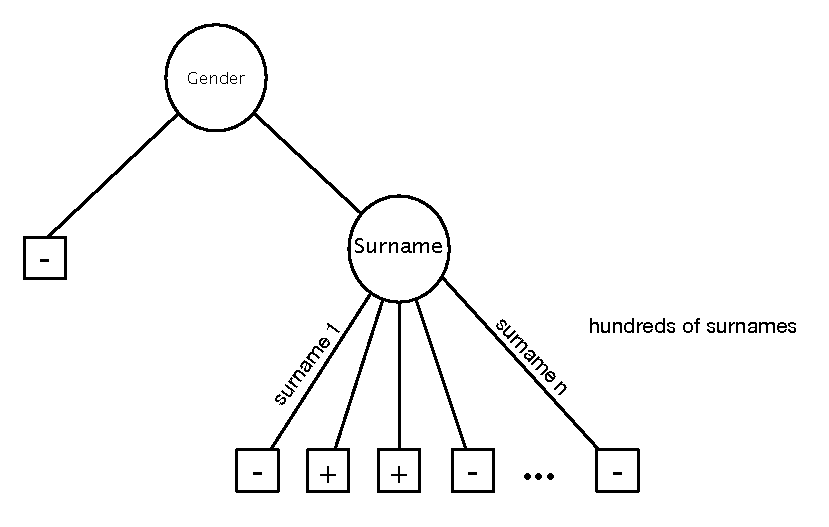
\includegraphics[width=\linewidth]{fig1.pdf}
	\caption{A decision tree for the basic features}
	\label{fig:tree_base}
\end{figure}

The above example illustrates that without additional knowledge, an induction algorithm will yield a very poor result. Even if we attempt to use standard feature generation approaches, there is no additional information that combinations of these features would find.
However, if we assume that we have access to a relational knowledge base connecting surnames to common countries of origin, we can begin to apply knowledge-based feature generation techniques to the problem, as we can move from the domain of surnames to that of countries. 

 Our goal is to separate this set of people to those at high risk and those at low risk using induction algorithms. We see that the existing feature set is insufficient to perform this task successfully. Therefore, our approach aims to construct new features for the learning task $T_1$ by recursively creating a new learning problem $T_2$. Once we have done so, we can use induction methods on $T_2$ in order to create a classifier that can be used in $T_1$. We construct $T_2$ as follows: 
  The training objects are surnames; surnames of people with the disease are labelled as positive. The features for these new objects are extracted from the knowledge base, they are their countries of origin.
Solving the above learning problem through an induction algorithm yields a classifier on surnames that distinguishes between surnames of patients with the disease and surnames of healthy individuals. This classifier for $T_2$ can then be used as a binary feature in the original problem $T_1$ by applying it to the feature value of surname. For example, it can be used as a feature in the node of value female in figure \ref{fig:tree_base}, yielding the tree seen in figure \ref{fig:lvl1_tree}. 

This new feature gives us a better generalization over the baseline solution, as we now abstract the long list of surnames to a short list of countries. We can see this as nodes in the classifier for $T_2$ are derived from multiple surnames. This result also allows us to capture previously unseen surnames from those countries. However, this is not a sufficient solution, as we have no way of generalizing on previously unseen countries of origin, and some countries may not have sufficient representation to induce an accurate classifier. %talk about not concept?


\begin{figure}
	\centering
	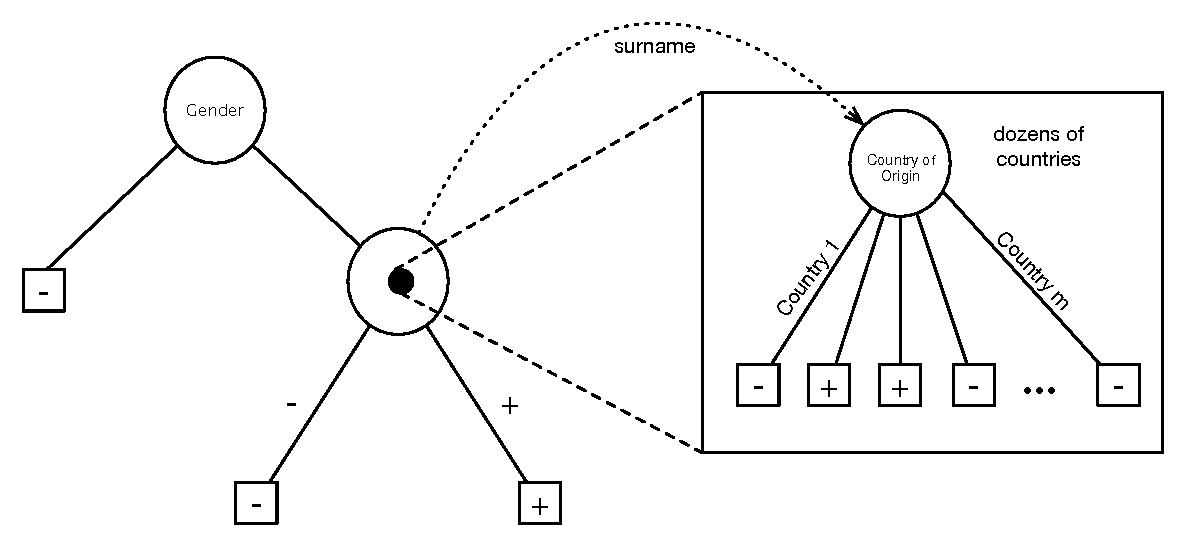
\includegraphics[width=\linewidth]{fig2.pdf}
	\caption{A constructed feature used within a decision tree}
	\label{fig:lvl1_tree}
\end{figure}

Once again, we require additional knowledge in order to capture the target concept of $T_2$. 
Therefore, we can recursively apply our method while trying to learn $T_2$ in an attempt to better locate the target concept and induce a classifier for $T_1$.
We create a new training set, the objects of which are countries of origin, with countries of surnames belonging to people with high risk are labelled as positive. The knowledge base regarding countries is then used to construct features for this new this training set, giving us a recursive learning problem $T_3$.

We can then use $T_3$ as an input to an induction algorithm. As a result of this process, we end up with a classifier for $T_3$, which tries to separate between countries of origin of people at risk and those not at risk. This classifier will do so by looking at the properties of countries, and reach the conclusion that countries with high average temperature and low precipitation: both being characteristic of desert areas.
This classifier is then used on the country of origin feature in $T_2$, yielding a new feature for $T_2$.  This new feature can then be used when inducting a classifier for $T_2$, which, as we have mentioned earlier, is used as a feature for the original problem $T_1$.

The complete process is depicted in figure \ref{fig:moving_to_lvl2}. The resulting two-level recursive classifier is depicted in figure \ref{fig:lvl2_tree}. This constructed feature allows us to concisely and accurately capture the target concept, as the construction process is guided by the target concept, in a manner similar to that of deductive approaches.
While this is a simple example, it illustrates how an unsolvable learning problem given the original features can be solved via the use of complex additional knowledge and existing induction methods.

%We also note that while an unsupervised approach can also create a combination of features that when used together allow us to identify the target concept, the unsupervised nature of the search makes such an attempt computationally expensive, especially when the knowledge base is extensive and multiple logical leaps are necessary.

\begin{figure*}[t]
	\centering
	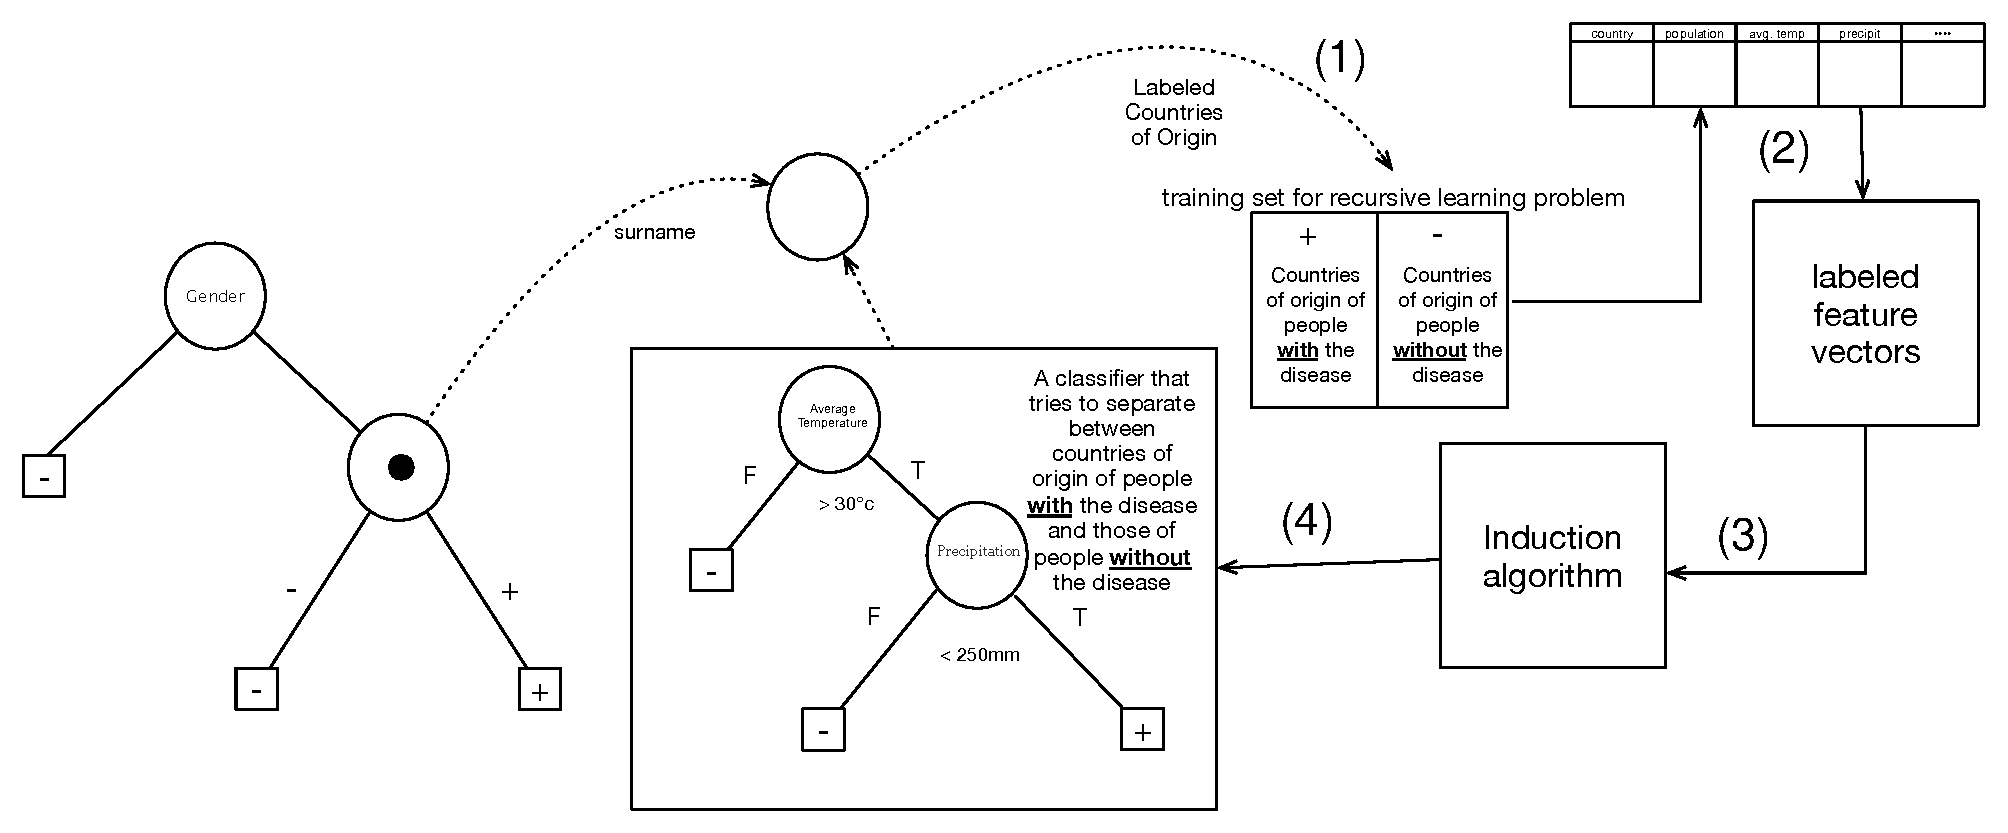
\includegraphics[width=\linewidth]{fig4_annotated.pdf}
	\caption{Recursive construction of a learning problem on countries of origin. $(1)$-Creating the objects for the new problem. $(2)$-Creating features using the knowledge base. $(3)$-Applying an induction algorithm. $(4)$-The resulting feature.}
	\label{fig:moving_to_lvl2}
\end{figure*}

\begin{figure*}[t]
	\centering
	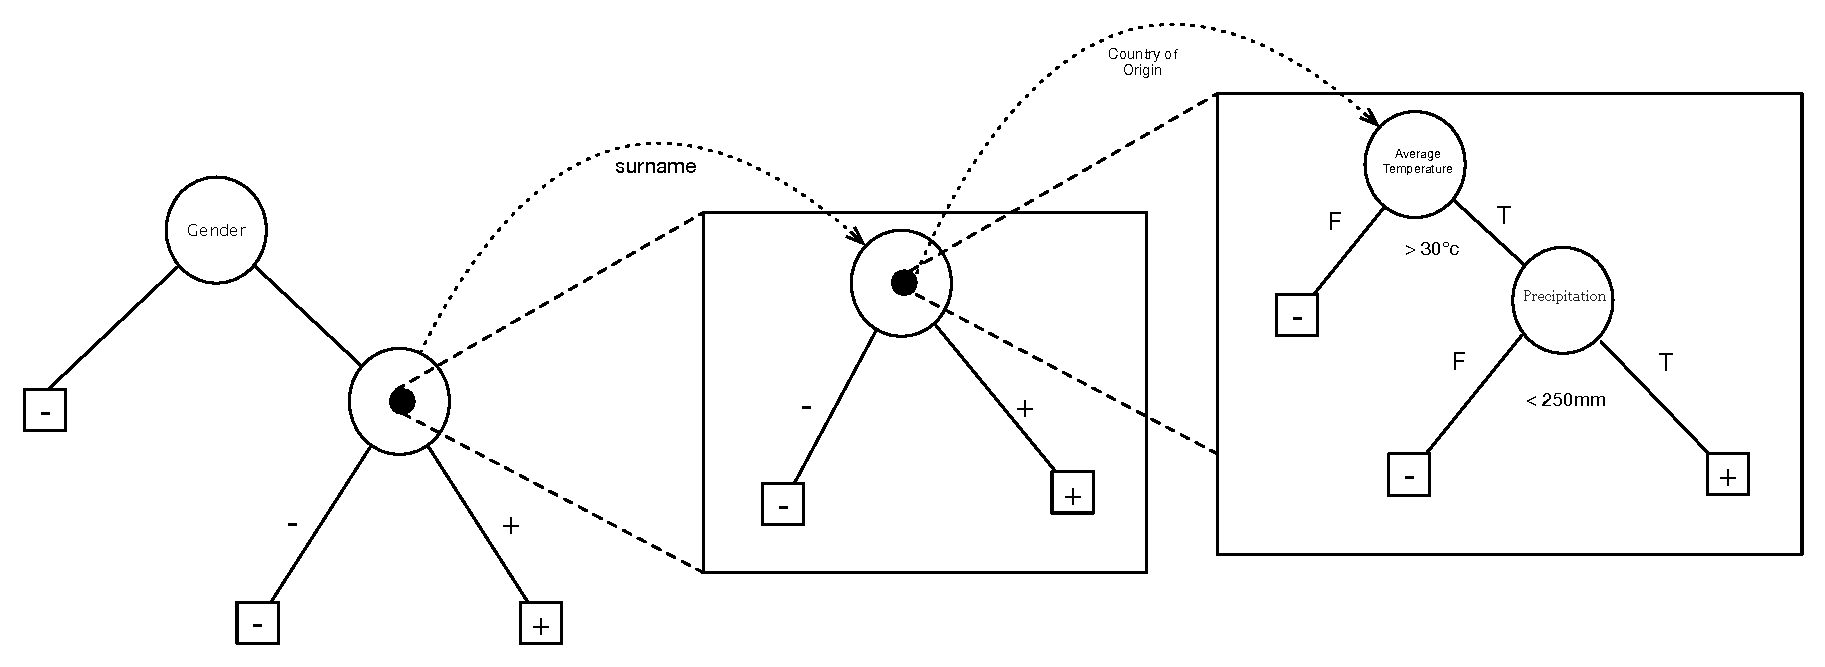
\includegraphics[width=\linewidth]{fig3.pdf}
	\caption{A two-level constructed feature used within a decision tree}
	\label{fig:lvl2_tree}
\end{figure*}


%%%%%%%%%%%%%%%%%%%%%%%%%%%%%%%%%%%%%%%%%%%%%%%%%%%%%%%%%%
%\section{Background} \label{background}
%%%%%%%%%%%%%%%%%%%%%%%%%%%%%%%%%%%%%%%%%%%%%%%%%%%%%%%%%%

%One of the earliest methods of utilizing relational information is \emph{Inductive Logic Programming(ILP)} \citep{quinlan1990learning, muggleton1991inductive}. This approach induces a set of first-order formulae that define a good separation of the given training set.
%Following this work, Relational Learning - techniques designed to utilize relational databases, have become increasingly prevalent. One such technique is that of View Learning \citep{davis2005view}, which generated new tables from existing ones, effectively performing feature generation for relational methods.

%One major attempt at adding relational knowledge to traditional induction algorithms was \emph{propositionalization} \citep{kramer2000bottom}: Since we wish to allow the use of first-order predicates in propositional methods, we create possible (non recursive) first-order predicates in a process known as refinement search \citep{van1998completeness}.
%We define a graph of possible first-order formulae by selecting an initial relation and allowing one of two possible refinement operators: The first operator is binding a single variable in the formula by assigning a constant value to it, and the second is binding a single variable using another relation.

%These operators define a search space. For each formula, we can ask whether a given object satisfies it, giving us a binary query for the data. We often prefer to only use formulae with one unbound variable, as it simplifies the satisfaction check.
%It is important to note that each application of refinement operators yields a formula that is subsumed by the parent, meaning that any object satisfying the child formula will also satisfy its parent.

%A major setback of this process is that it generates an impractically large number of features, most of which irrelevant.  To this end, \emph{upgrade} methods such as ICL \citep{van2001upgrade} were suggested, where instead of creating predicates a-priori, we do so during the training phase, allowing us to avoid searching non-promising refinements.

%As a continuation to this trend, \citet{popescul200716} suggest SGLR, an upgrade method which allows the generation of nominal attributes by using aggregation operators. Essentially, instead of simply checking whether a first-order predicate is satisfied, we perform aggregation over all objects which satisfy it. In addition, SGRL offers an initial insight into the issue of improving the search process by using Akaike's information criteria (AIC, see \citet{burnham2002model}) to select features based on a combination of complexity and predictive power.

%In the case where this external knowledge is organized as a set of relations between entities, several methods can be used. One such method is using \emph{Inductive Logic Programming} \citep{muggleton1991inductive} to generate features, in a process referred to as \emph{upgrading} \citep{van2001upgrade}. This is demonstrated through the ICL algorithm, which uses a refinement graph to search for logical formulae which serve as features. The SGLR algorithm \citep{popescul200716} extends this idea to numerical features, generated using aggregation-based techniques, and then utilizes regression for inference.

%TODO: this section to talk about propo as chain of joins? add that needs serious filtering/subsampling to be tractable, and give newish citations (proposizitonaliztion: wordification blah blah paper?)
%%%%%%%%%%%%%%%%%%%%%%%%%%%%%%%%%%%%%%%%%%%%%%%%%%%%%%%%%%
%\section{Using relational knowledge to generate features: A traditional approach}
%%%%%%%%%%%%%%%%%%%%%%%%%%%%%%%%%%%%%%%%%%%%%%%%%%%%%%%%%%
%Before we discuss our approach, it is prudent to consider existing techniques for turning relational knowledge into additional features.
%Discuss propositionalization?

%%%%%%%%%%%%%%%%%%%%%%%%%%%%%%%%%%%%%%%%%%%%%%%%%%%%%%%%%%
\section{Generating Features through Recursive Induction} \label{formal}
%%%%%%%%%%%%%%%%%%%%%%%%%%%%%%%%%%%%%%%%%%%%%%%%%%%%%%%%%%

We begin our discussion with the standard definition of an induction problem. 
Let $O$ be a set of objects. Let $Y=\{0,1\}$ be a set of labels \footnote{We assume binary labels for ease of discussion}. Let $C:O\rightarrow Y$ be the target concept. Let $S=\{(o_{1},y_{1}),\ldots,(o_{m},y_{m})\}$ be a set of labelled examples such that $o_{i}\in O, y_{i}\in Y, C(o_i)=y_i$. 
Let $F=\{f_{1},\ldots,f_{n}\}$ be a \emph{feature map}, a set of \emph{feature functions} $f_{i}:O\rightarrow I_{i}$.  This definition implies a training set represented by feature vectors: $S_F=\{ (\langle f_1(o_i),\ldots,f_n(o_i)\rangle, y_i) | (o_i,y_i) \in S\}$. A learning algorithm $L$ takes $S_F$ as inputs, and outputs a classifier $h_{S_F}:O\rightarrow Y$.
\begin{defn}
	Let $L(S,F)=h_{S_F}$ be the classifier outputted by $L$ given $\langle S,F\rangle$. Assuming $S\sim\ D$, the generalization error of a learning algorithm $L$ is the probability $Pr(h_{S_F}(x)\neq y)$, where $(x,y)\sim\ D$.
\end{defn}

%The general task of Feature Generation is as follows: Given $\langle S,F\rangle$, construct a new feature map $F'$ such that when we use an induction algorithm to find a hypothesis, it will do so more effectively. More formally, we require that $Sum(o\in O,h_{S_F}(o)\neq C(o)) \geq Sum(o\in O,h_{S_F'}(o)\neq C(o))$. Usually, the same induction algorithm is used on both $F$ and $F'$, allowing for a controlled comparison which lowers the impact of the induction algorithm. 

In this work, we assume that in addition to $S_F$ we also have a set of binary \footnote{If our relations are not binary, we can use projection to create multiple binary relations instead} relations ${\cal R}=\{R_{1},\ldots,R_{t}\}, R_j:D_j\times D_{j'}$ representing our knowledge base. 
\begin{defn}
	A \emph{supervised feature generation algorithm} $A$ based on ${\cal R}$ is an algorithm that given $\langle S,F,{\cal R} \rangle$, creates a new feature map $F_{{\cal R}}=\{f'_{1},\ldots,f'_{l}\}, f'_{k}:O\rightarrow I_k$.
\end{defn}

In order to evaluate the output of a feature generation algorithm $A$, we must define its utility. Given $\langle S,F \rangle$, $A$ generates a feature set $F'_A$.
Given $S\sim\ D$, a feature set $F$, a generated feature set $F'_A$ and a learning algorithm $L$, the utility of $A$ is $U(A(S,F))=Pr(h_{S_F}(x)\neq y)-Pr(h_{S_{F'_A}}(x)\neq y)$, where $(x,y)\sim\ D$.

The implications of this definition are twofold: First, if the classifier induced by $L$ given  $\langle S,F \rangle$ yields a low generalization error, there is little to be gained through feature generation. Second, in order for the utility of $A$ to be positive, the generated feature set $F'_A$ must yield lower generalization error than $F$.

When using a feature generation algorithm using a set of relations ${\cal R}$, we would like to achieve a higher utility than that achieved without the use of ${\cal R}$. Clearly, in order to do so we must require some connection between ${\cal R}$ and our feature set $F$. To that effect, we add an additional requirement:  $\bigcup_{f_i} I_i \cap \bigcup_{R_j} D_j \neq \emptyset$. 

\subsection{An unsupervised approach to knowledge-based feature generation} \label{shallow_section}

To begin with, we shall try to ignore the labels, and define an unsupervised feature generation algorithm based on ${\cal R}$. We call this algorithm \emph{Shallow}, as it uses the relations in a shallow manner to create features. Using \emph{Shallow}, we can highlight several important concepts of our approach.

Let us first consider the case where any given relation $R_j$ is a function $R_j:D_j\rightarrow D_{j'}$. In this case, for any given $f_i,R_j$ such that 
$Image(f_i) \subseteq D_j$, we can compose $R_j$ onto $f_i$, giving us a function $f_{i,j}(x)=R_j\circ f_i=R_j(f_i(x)),f_{i,j}:O\rightarrow D_{j'}$. For example, if $f_i$ lists a person's country of origin, and $R_j$ maps countries to their continent, then $f_{i,j}$ lists a person's continent of origin.
Under this condition, we can define the new feature set using a closed formula: $\{f_{i,j}|Image(f_i) \subseteq D_j\}$.

Now that we have considered the simple case, we can consider more complex cases.
For one, we must consider the case where $Image(f_i) \not\subset D_j$ but $Image(f_i) \cap D_j \neq\emptyset$. In this case, there are values for which $R_j$ cannot be applied. We can therefore treat $R_j$ as a partial function from $Image(f_i)$ to $D_{j'}$. In order to complete this partial function, let us first mark \emph{undefined} as $\perp$. We can turn $R_j$ into a full function with regards to $Image(f_i)$ as follows: $\tilde{R}_j(x)=\begin{cases} R_j(x) &\mbox{if } x\in D_j\\ 
\perp & \mbox{otherwise } \end{cases}$.
The result is a full function $\tilde{R}_j:Image(f_i)\cup D_j\rightarrow D_{j'}\cup\{\perp\}$. We also note that the same process can be applied in cases where $R_j$  has missing values, meaning it is a partial function with regards to $D_j$

Although there are many relations which are also functions, such a requirement may serve as a limitation. For example, a relation mapping a surnames to their countries of origin, as in section \ref{motivation}, may have multiple countries of origin for a single surname. Similarly, a relation mapping a parent to their children may have many children for the same parent.
In cases such as this, composing $R_j$ onto $F_i$ may yield a set of values, requiring an aggregation function to be used should we wish to utilize it effectively. There are many possible aggregation functions that we can apply on such a value set, but we shall discuss three major ones:
\begin{itemize}
	\item All- Given a set of values, whether they all fulfil a certain predicate $p:D_{j'}\rightarrow\{0,1\}$.
	\item Exists- Given a set of values, whether there exists a value in that set which fulfils a certain predicate $p$.
	\item Majority- Given a set of values, whether a majority of them fulfil a certain predicate $p$.
\end{itemize}
All of the above require a predicate function $p:D_{j'}\rightarrow \{0,1\}$.
As an example, we can check whether a constant $c\in D_{j'}$ is within the values of the set by using $p(x)=\begin{cases}
1 & \mbox{if } x=c\\ 0 & \mbox{otherwise}
\end{cases}$ alongside the ``exists" aggregation method.

In some situations, we would like to work with binary features rather than multi-valued ones. In such cases, we can restrict the constructed $f_{i,j}$ by a constant, yielding $f_{i,j,c}(x)=\begin{cases}
1 & \mbox{if } f_{i,j}(x)=c\\
0 & \mbox{otherwise}
\end{cases}$. In the more complex cases, we must consider how to handle missing values and multiple values. To simplify, we can handle $\perp$ as false and use the ``exists" aggregation condition to handle these cases.

Now that we have considered all possible behaviours of a given relation $R_j$, we can proceed to define the \emph{Shallow} algorithm. Given a feature $f_i$, \emph{Shallow} will go over the relations within the knowledge base and attempt to create features $f_{i,j,c}:O\rightarrow D_{j'}\cup\{\perp\}$ through the discussed techniques. \emph{Shallow} then gathers all generated features and outputs them. The pseudo-code is given below.

\begin{algorithm}[H]
	\caption{\emph{Shallow}: Non-recursive Feature Generation using relations}
	\label{code-compete}
	\small
	%insert param stuff
	\begin{algorithmic}
		\Function{CreateFeatures}{$S$,$F$, ${\cal R}$}
		\State $F_{result}=\emptyset$
		\For {$f_i \in F$}
		\For {$R_j \in {\cal R}$}
		\If {$Image(f_i)\cap D_{j}=\emptyset$}
			\State Continue
		\ElsIf {$R_j:D_j\rightarrow D_{j'}$ and $Image(f_i)\subseteq D_{j}$}
			\State $F_{result}=F_{result}\cup \{f_{i,j}=R_j\circ f_i\}$
		\ElsIf {$R_j:D_j\rightarrow D_{j'}$ and $Image(f_i)\cap D_{j}\neq\emptyset$}
			\State $F_{result}=F_{result}\cup \{f_{i,j}(x)=\begin{cases} R_j( f_i(x)) &\mbox{if } f_i(x)\in D_j\\ 
			\perp & \mbox{otherwise } \end{cases}\}$
		\Else \Comment $R_j$ is a relation $R_j:D_j\times D_{j'}$
		\State $F_{result}=F_{result}\cup \{Aggregate(p,f_{i,j})\}$
		\EndIf
		\EndFor
		\EndFor
		\State \Return $F_{result}$ 
		\EndFunction
		
	\end{algorithmic}
\end{algorithm}

We see that this approach allows us to generate features from our knowledge base, regardless of the ways in which it interacts with our existing features. One example of such features is that of semantic type, features making use of the ``IS-A" relation to note the entity type. We note that this approach creates a potentially large number of features, and that a given feature may have a large number of values. While this approach does allow us a degree of generalization, it can only utilize our knowledge base shallowly, from base entities to their values. 
Should we try to apply a chain of relations rather than a single one, we can begin to explore more complex domains. However, we must consider the exponential nature of such a chain. Without any way to guide our search through the knowledge base, we are likely to generate and increasingly large number of relations, many of which will be irrelevant. 

\subsection{Creating Learning Problems using Relations} \label{algorithm_section} 

%todo: switch to main flow->branches. make sure the alg shows all the cases!

Now that we have seen how an unsupervised algorithm would make use of a knowledge base for feature generation, we may begin to properly discuss our approach. To do so, we must understand how our approach creates new induction problems using the knowledge base.

Given an existing feature $f_{i}:O\rightarrow Dom_i$, our algorithm will formulate a new learning task trying to separate values in $Dom_i$ associated with positive examples of the original learning task from those appearing in negative ones. The result of the new learning task will be a classifier
$h_{i}:Dom_{i}\rightarrow Y$ which we can then use to label elements in $Dom_i$, such as those appearing in $f_{i}$. We can then define a new feature $f'_{i}(x)=h_{i}(f_{i}(x)), f'_{i}:O\rightarrow Y$.
We name this algorithm \emph{FEAGURE} (FEAture Generation Using REcursive induction). The full pseudo-code is described in algorithm \ref{code-creating-prob}.

In order to explain how we create such $h_{i}$, let us first consider the creation of a new learning problem. Once we have done so, we can use any induction algorithm to create $h_i$. 
Given a feature $f_{i}$, we first define $v_i(S) = \{v | (o,y) \in S, f_{i}(o)=v\}$ the set of feature values for $f_i$ in $S$. In the intro example, for instance, $v_i(S)$ will b
e the set of all last names of patients that appeared in the training set.
We use $v_i(S)$ as our set of objects. To define a learning problem, we must consider their labels. 

In the simple case, every feature value appears only for a single example in $S$. In that case, we can simply take the same label, with the result being $label(v)=y$ where $f_i(x)=v,(x,y)\in S$. In the above example, if each patient has a unique surname, each surname would be labelled according to that patient's label.
Most features in general, and in machine learning tasks in particular, however, do not have a unique value for each example. In such cases we would have multiple examples in $S$ such that $f_i(x)=v$. Let us call $S(v)$ the set of such examples. In order for us to give a label for $v$, we must aggregate the labels of objects in $S(v)$ somehow. As in section \ref{shallow_section}, we can consider three major aggregation functions.
Using the All aggregation function results in a strict labelling, as a value will be classified as belonging to the target concept only if all examples in which that value has appeared are labelled positive. The result is the consistent label function: $label(v)=\begin{cases} 1 &\mbox{if } \forall (x,y)\in S(v): y=1\\ 
0 & \mbox{otherwise } \end{cases}$.
 A more lenient label function is the majority label, taking the Majority aggregation function: $label(v)=majority(\{y|(x,y)\in S(v)\})$.
 In the intro example, the consistent label would take the set of patients with the given surname, and label that surname as having high risk only if all such patients have the disease. The majority label, in comparison, would check whether most patients with that name have the disease.
 
We now formulate a new learning problem with the constructed training set
$S'_i = \{ (v, label(v)) | v \in v_i(S) \}$.
To fully define our learning problem, we must specify a feature map over $v_i(S)\subseteq Dom_i$. Consider a relation $R_j$ such that $D_j\cap v_i(S)\neq \emptyset$. For such $R_j$, if it is a function, we can simply use it as a feature function, or restrict by a constant $\left(f_{j,c}(v)=\begin{cases} 1 &\mbox{if } \ R_j(v)=c\\ 
0 & \mbox{otherwise } \end{cases}\right)$. If $R_j$ is a partial function, we simply have a feature with missing values. Finally, if $R_j$ is not a function, we can use aggregation as in section \ref{shallow_section} to create features.

Once we have considered all relations in ${\cal R}$, we can generate a feature map for $S'_i$. Given $R_j$, assuming it is relevant to the problem domain, meaning $v_i(S)\cap D_j\neq\emptyset$, we can utilize it as a feature. We then look at all constants $c\in \{R_j(v)|v\in v_i(S)\land R_j(v)\neq \perp\}$. For each such $c$, we add $f_{j,c}:Dom_i\rightarrow \{0,1,\perp\}$ to our feature map. 
For example, in the intro example, each constant $c$ is a country of origin.
The result of this process is a feature map for $S'_i$, $F_{\cal R}$ which includes all such $f_{j,c}$. We now have a complete induction problem for which we can train a classifier, giving us $h_i:Dom_i\rightarrow Y$. We can then use this $h_i$ on objects in $S$ as discussed above, giving us $f'_{i}(x)=h_{i}(f_{i}(x)), f'_{i}:O\rightarrow Y$. 

We note that once we have an induction problem over $Dom_i$, we can apply our approach recursively on $S'_i$ in order to create additional features. We can see an example of this in section \ref{motivation}, wherein we construct a second-level problem on countries of origin to correctly identify the appropriate conditions that signify high risk countries.
 For each relation $R_j$, rather than restricting it via constants, we take all values of it, and treat those as a feature $f_j(v)=\{v'|R_j(v)=v' \lor v'\in R_j(v) \}$. Assuming $R_j$ is a function or partial function, $f_j$ will also be a function or partial function respectively, and we can then construct a learning problem over values $f_j$ in the same manner as before, yielding a classifier $h_j:D_{j'}\rightarrow Y$, which can then be used to create a feature for $S'_i$. 
 
 In cases where $R_j$ is a relation, $f_j(v)$ is a set of values- a relation. In such cases, We must discuss both how to extract a new learning problem, and how a classifier is then used for a set of features.
 To begin with, let us tackle the issue of constructing a learning problem where each feature value is a set. In such cases, we still have the above problem where multiple examples may contain the same value, but a single example has multiple values. A simple solution to this issue is to give each value the same label as that of the example, and proceeding to resolve multiple labels via aggregation as we have discussed previously. 
 Once we have done so, we can construct a new learning problem for $f_j$ and, using FEAGURE, receive a classifier $h_j:D_{j'}\rightarrow Y$.
 Another question we must ask ourselves is how such a classifier can be applied to the set of values in $f_j(v)$. To illustrate, consider the classifier shown in figure \ref{figure5}. We see that the classifier can be applied to multiple values of the feature, giving us a set of labels as the label of our example. As we have already discussed how such a set of labels should be resolved when discussing the labelling of the constructed learning problem, we can apply the same solution here, giving us a single feature value for our example in $S'_i$.

\begin{figure}[t]
	\centering
	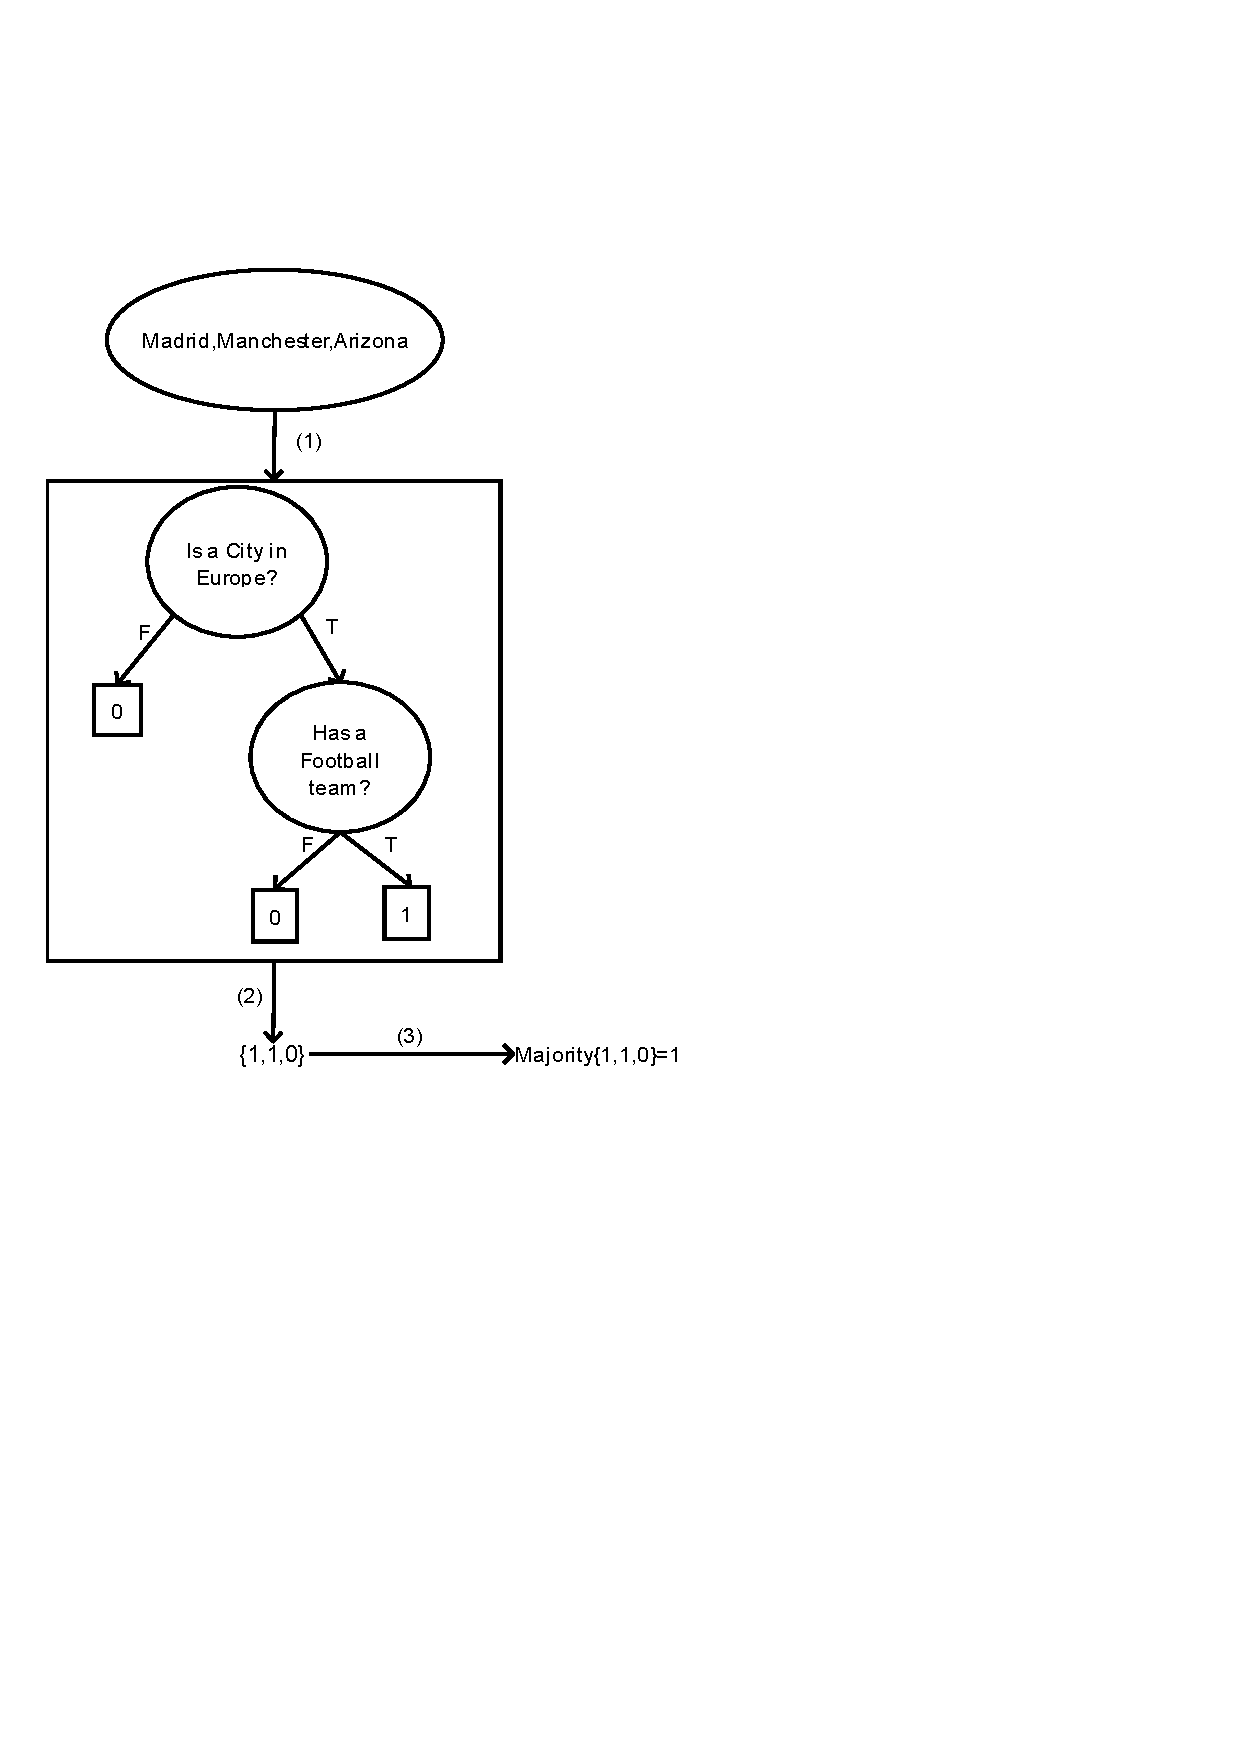
\includegraphics[scale=0.8]{fig6.pdf}
	\caption{Using a constructed classifier on a set of values: $(1)$-Feature values are used to construct a learning problem. $(2)$-The classifier is then applied to each value. $(3)$-An aggregation function is applied on the results. In this case, the majority function is used to determine the output for the learning problem.}
	\label{figure5}
\end{figure}

In many feature generation approaches, feature selection methods play a key part in filtering out poor features. In FEAGURE, we can use feature selection both as a filtering mechanism, as well as a search parameter.
As a filtering technique, the features generated by FEAGURE are compared to the already existing feature map $F$. There is a multitude of feature selection techniques that can be applied for this task, but we shall cover three filtering criteria.
\begin{enumerate}
	\item Maximal Information Gain (IG)- The information gain metric \cite{quinlan1986} compares how well a single feature reduces the amount of information entropy within a given labelled set should we split by it. In essence, it measures how well each feature separates the set based on its labels. Taking the maximal information gain as a metric, we measure whether the constructed feature gives a better separation compared to all existing features in $F$.
	\item Average Information Gain- Just as we can compare our feature to the maximal IG of the feature map, we can compare it to the mean IG for features in $F$.
	\item Sufficient Diversity- IG based approaches measure the separation of the training set. In many feature generation tasks, however, the more correct approach is to generate features which differ from existing features. To do so, we could require that the correlation of the generated feature with features in $F$ be below a certain threshold.
\end{enumerate}
Beyond their use for filtering, criteria that measure the performance of features such as the ones above can be used as a deciding factor in whether or not a constructed learning problem should apply FEAGURE recursively. The idea here is that should the generated feature be close to the threshold, we may wish to continue expanding it in hopes of giving it the necessary boost.

\begin{algorithm}[H]
	\caption{FEAGURE-FEAture Generation Using REcursive induction}
	\label{code-creating-prob}
	\small
		%insert param stuff
		\begin{algorithmic}
			\Function{ConstructFeatures}{$F$, $S$, ${\cal R}$}
				\For {$f_i\in F$}
				\State $S'_i,F_{\cal R}$= \Call{CreateNewProblem}{$f_i$,$S$,${\cal R}$} \Comment{We can apply our algorithm recursively here}
				\State $h_i$= \Call{InductionAlgorithm}{$S'_i,F_{\cal R}$} 
				\If {\Call{Compare}{$h_i,F$}} \Comment Compare $h_i$ to $F$
				\State add $h_i$ to new features
				\EndIf
				\EndFor
				\State \Return new features
			\EndFunction
			\State 
			\Function{CreateNewProblem}{$f_{i}$, $S$, ${\cal R}$}
                \State $v_i(S) = \{v | (o,y) \in S, f_{i}(o)=v\}$
                \State $S'_i = \{ (v, label(v)) | v \in v_i(S) \}$ 
                \Comment $label(v)$ can be, for example, the majority function.
                \State Let $f_{j,c}(v)=\begin{cases} 1 &\mbox{if } \ R_j(v)=c\lor c\in R_j(v) \\ 
                \perp & \mbox{if} R_j(v)=\perp\\
                0 & \mbox{otherwise } \end{cases}$
                \State $F_{\cal R}=\{f_{j,c}| c\in D_{j'}, R_j\in{\cal R}\}$
                \State \Comment We only need $c$ such that $\exists v\in v_i(S):f_{j,c}(v)=1$
                \State \Return $S'_i, F_{\cal R}$ 
			\EndFunction
			
		\end{algorithmic}
	\end{algorithm}

We note that this feature generation approach creates features which can be used alongside any induction algorithm. Additionally, any induction algorithm can be used to learn $h_i$. Due to this generality, the extensive knowledge and literature available for induction methods applies in full. Furthermore, the recursive nature of FEAGURE allows for a structured search of the knowledge base, with each new recursive problem modelling a projection of the problem space to the new domain, allowing for a process similar to deductive learning. For example, in the motivating example, we began by learning a problem regarding patients, which we projected to a new domain of surnames. We then re-contextualized that problem to the domain of countries, for which we located a good solution. We then used this solution to resolve the original learning task.

While this approach has many benefits, there are is a potential issue with this approach, namely, that the number of features generated by it is limited to the number of features in the original problem. There are several methods to resolve this issue:
\begin{enumerate}
	\item Using multiple induction algorithms on the generated learning problem may yield significantly different classifiers which can then be used as unique features, in a manner resembling an ensemble approach.
	\item Use of feature selection methods within the generated problem allows for multiple classifiers to be learned by reusing the same feature map. This approach has the potential downside that later features may be significantly worse.
	\item Some induction algorithms, the chief of which being decision tree classifier induction methods, yield decomposable classifiers. In the case of decision trees, such a tree classifier can be flattened into a set of decision stumps, each holding a single split of the tree. This approach allows us to turn a single strong feature into multiple weaker ones.
	\item By sub-sampling our training set, we can learn features that only apply to a part of the training set, thus potentially giving us different, local features.
\end{enumerate}

%\subsection{Creating Multiple Features} \label{multi_feature}

%Now that we have discussed how we create a single feature, we must consider how to expand this and generate multiple features. One simple approach would be to simply apply the above technique (algorithm \ref{code-creating-prob}) once for each feature.
%Naturally, this would result in $n$ new features.
%Even if we apply the above approach recursively, we would still obtain only $n$ new features, though they may be stronger as we have generated new features within each learning problem.
%Thus, if we wish to generate a larger number of features, we must take a different approach.

%While most traditional machine learning algorithms yield useful properties such as filtering and regularization, a Decision Tree classifier offers several useful traits with regards to recursive application of our approach:
%\begin{enumerate}
%	\item Decomposability: A Decision Tree classifier can be easily decomposed into multiple Decision Stumps, allowing us to decide between generating a single strong feature or multiple weaker features.
%	\item Interpertability: Decision trees are generally considered easier to interpret and understand, allowing us to easily grasp which relations are more impactful, and thus which domains are likely to contain additional knowledge which we may not have utilized.
%	\item Orthogonality: Since features further down in a decision tree are orthogonal to ones already used, we can effectively limit our search space, as relations we have already used will not be picked. This also has a beneficial side effect of increasing variety in generated features.
%\end{enumerate}

\subsection{Finding Locally Improving Features} \label{tree_usage}

As we have previously discussed, in some cases creating multiple features is superior to generating only a few. Beyond this, in many cases it is far easier to locate powerful features within a localized subset of data which shares common attributes rather than trying to locate the same features in a more global context. In the motivating example, for instance, male patients are irrelevant to the target concept, and thus could potentially cause noise when used for feature generation.
There is a multitude of approaches to creating such local features. We shall look at a few of these approaches:
\begin{itemize}
	\item Sub-Sampling: By sampling a subset of training examples, we can hope to create a good local context for feature generation. An issue with this approach is that there is a huge number of possible subsets, and thus going over all of them is not computationally feasible. 
	\item Clustering: This approach attempts to make use of the feature set to create clusters of similar examples. In some cases, this would indeed yield good local contexts, but this approach is potentially problematic for our algorithm, as it is very likely that similar examples will have the same label, thus creating highly unbalanced learning problems, which would be more difficult to utilize effectively.
	\item Divide \& Conquer: This approach seeks to iteratively create increasingly smaller subsets of the original problem by dividing the problem according to the values of a feature. Most often, the IG metric is used to determine the feature used to split the examples.
\end{itemize}

Of the above approaches, the Divide \& Conquer approach yields numerous advantages we can make use of, namely:
\begin{enumerate}
	\item Orthogonality: Because all examples with the same value for a given feature are grouped together, any further splits must make use of different features. Due to this and the fact that the features selected in each step have high IG, it is usually the case that features chosen later in the process will be mostly orthogonal to previously chosen features. This results in a larger variety of features overall. In our approach in particular, the elimination of a feature prunes the search tree and forces later splits to rely on different features and thus different domains.
	\item interpertability: Looking at the features used at each splitting point gives us an intuitive understanding of the resulting subsets. Because of this, we can more easily understand why certain features were picked over others, which domains are no longer relevant, and so on.
	\item Iterative construction: The divide \& conquer approach allows for an iterative search process, which we can then easily interrupt if a sufficient number of features were generated, or when the remaining training set is no longer sufficiently representative for drawing meaningful conclusions.
	\item Guided by labelling: This approach explicitly uses the labels of the training set to create meaningfully different groups. As a result of this, we can expect that as we go further down, the need for good, distinguishing features will rise, and we can locate stronger features.
\end{enumerate}

Due to the above advantages, we have a strong incentive to utilize the divide \& conquer approach when attempting to create additional features using FEAGURE. This new algorithm, which we shall name \emph{Deep-FEAGURE}, begins by taking the entire training set and applying FEAGURE to it. Once features have been generated, any generated features which have performed well are kept, and the feature with the highest information gain (potentially the one generated by FEAGURE) is used to split the training set into groups according to its values.
For each of these new, smaller training sets we then repeat this process until we either receive a consistent training set, meaning all examples have the same label, or the size of the training set becomes so small that it is wholly unrepresentative of the complete problem.
Once we have finished this process, only the generated features are kept, and returned as the output of Deep-FEAGURE.

A major potential issue that must be considered in any induction approach, and is especially problematic for divide \& conquer approaches, is that of over-fitting, meaning that the result is too adjusted to seen data, and cannot generalize for previously unseen data. In the extreme case, an induction method may yield a classifier that simply memorizes the known data. This classifier will yield perfect results for seen data, but is worthless for unseen data.
To combat this issue, we consider several steps:
\begin{itemize}
	\item Limiting the minimal size of the training set allows us to control for unrepresentative subsets, which is a major factor in over-fitting.
	\item Feature selection inherent to FEAGURE limits the potential for over-fitting, as generated features must be beneficial to enter the feature pool. It is important to mention, however, that a very strict feature selection criterion may have an opposite effect, as any feature that pass it must be very well fitted to the training data.
	\item Limiting the depth of search by refusing to further split beyond a certain depth is another way to prevent unrepresentative subsets. Of particular notice, the number of relations in our knowledge base gives us a natural depth limit due to the orthogonal nature of this approach. Essentially, once a certain relation has been used, it is unlikely that another feature down the tree will make use of it again, as we have already split the training set according to values of that domain. 
	\item Well-known induction approaches often acknowledge the issue of over-fitting, and offer multiple techniques to minimize it. Should we use search trees, for example, flattening can be used to create a set of weaker features, which is less likely to over-fit than a single complex decision tree.
\end{itemize}

\begin{algorithm}[H]
	\caption{Deep FEAGURE- Divide \& Conquer Feature Generation}
	\label{code-tree-thing}
	\small
		minSize- minimal size of a node.

        SplitByFeature- a method that splits a training set according to a feature.
        
		\begin{algorithmic}
			\Function{ConstructFeaturesInANode}{$S$, $F$, ${\cal R}$}
                \If {$|S|<$minSize} 
                    \State
                    \Return 
                \EndIf
                \State newFeatures=\Call{FEAGURE}{$S$, $F$, ${\cal R}$}
                \State $f_{best}$=\Call{bestFeature}{$S$,$F\cup$ newFeatures}
                \State \Return \Call{SplitByFeature}{$S$, $f_{best}$}, newFeatures
			\EndFunction

            			
			\State 
            \Function{ConstructFeatures}{$S$, $F$, ${\cal R}$}
                \State currentFeatures= $\emptyset$
                \State sons, $F_{new}$=\Call{ConstructFeaturesInANode}{$S$, $F$, ${\cal R}$}
                \State currentFeatures= currentFeatures$\cup F_{new}$
                \For {son in sons}
                    \State newFeatures=\Call{ConstructFeatures}{son.$S$,$F$,${\cal R}$}
                    \State currentFeatures= currentFeatures$\cup$newFeatures
                \EndFor
                \State \Return currentFeatures
			\EndFunction
		\end{algorithmic}
	\end{algorithm}

%%%%%%%%%%%%%%%%%%%%%%%%%%%%%%%%%%%%%%%%%%%%%%%%%%%%%%%%%%
\subsection{Application of FEAGURE for Text Categorization}
%%%%%%%%%%%%%%%%%%%%%%%%%%%%%%%%%%%%%%%%%%%%%%%%%%%%%%%%%%

A particually interesting problem domain is that of \emph{Text Categorization}.
The text categorization problem is defined by a set of texts $O$ labelled by a set of categories $Y$ \footnote{We can assume $Y=\{0,1\}$ for ease of analysis}
 such that we create $S=\{(o_i,y_i)|o_i\in O, y_i\in Y\}$. Given $S$, The learning problem is to find a hypothesis $h:O\rightarrow Y$ which minimizes error over all possible texts of the given categories. To measure this error, a testing set is used as an approximation.
The standard approach to solving this problem is based on the bag-of-words \cite{Wu:1981:CST:1013228.511759,salton1983introduction} approach, which uses the frequencies of word appearances (without regards to order) within the text as features. 

Another way to describe this approach is that it creates a single feature, the titular bag-of-words, whose value is the set of all unique words in the text.
As we are well aware, however, not all words have semantic meaning. This observation makes usage of knowledge-based approaches non-trivial, as most knowledge bases rely on semantically meaningful entities rather than raw words.
To resolve this issue, we can make use of techniques such as Named Entity Recognition (NER), Wikification \cite{bunescu2006using} and Entity Linking \cite{rao2013entity}. These methods as well as similar techniques allow us to link words in the text with semantically meaningful entities. They do so by identifying keywords, linking related concepts, and other supervised and unsupervised techniques.
Using these techniques, we can move to a \emph{bag-of-entities}, that is, a model of the semantically meaningful entities within the text, without regard to order.

As discussed, we have seen the recent rise of Semantic Linked Data as a powerful knowledge base for text-based entities, with large databases such as Google Knowledge Graph \cite{pelikanova2014google}, Wikidata \cite{vrandevcic2014wikidata} and YAGO2 \cite{hoffart2013yago2} becoming common. 
These knowledge bases represent semantic knowledge through the use of relations, mostly represented by triplets of various schema such as RDF, or in structures such as OWL and XML. These structures conform to relationships between entities such as "born in", as well as type information.
Naturally, we would like to make use of such semantic data to improve upon the bag-of-words approach, with the implicit assumption that additional Semantic knowledge will allow us to better approximate the relationship between the text and its given category.

A major topic to consider when trying to apply FEAGURE to this domain is the fact that the bag-of-entities approach inherently creates features with many values. Because of this, special care must be taken to both the construction of recursive problems (a single example may have multiple applicable values) and the application of the resulting classifier on the document (several entities may apply).
Naturally, many entities within a given document will not apply to a given relation, and thus yield a value of $\perp$. To combat this, we only give a document the value of $\perp$ if it contains no entities which are relevant to the classifier.


%%%%%%%%%%%%%%%%%%%%%%%%%%%%%%%%%%%%%%%%%%%%%%%%%%%%%%%%%%
%\section{Discussion and Analysis of the FEAGURE algorithm}
%%%%%%%%%%%%%%%%%%%%%%%%%%%%%%%%%%%%%%%%%%%%%%%%%%%%%%%%%%

%tree in outer allows looking at 1 feature a time->more structured search

%We note that in order to prevent cycles which provide no new information, we do not allow the use of any relation that is the inverse of a previously used relation.

%The process of re-labelling and constructing recursive problems as detailed in section \ref{algorithm_section} offers some unique contributions:
%\begin{itemize}
%	\item By moving our domain space when constructing a new problem, we essentially look at the problem from another perspective, which allows for the discovery of complex relationships.
%	\item The process of re-labeling allows noise reduction and emphasizes more general trends within the data that may be harder to otherwise notice.
%	\item We can exploit the power of existing, well-developed learning algorithms when we create a classifier, and possibly use different ones as we take recursive steps.
%\end{itemize}
%Furthermore, we note that FEAGURE can locate locally useful features which may be difficult to identify when looking at the dataset as a whole.

%The resulting features of the FEAGURE algorithm %TODO: discuss that they are classifiers on feature values. also talk on the fact that we expect a few powerful&complex features, rather than many simple ones

%In terms of runtime performance, while FEAGURE has a large overhead, we note two major things: Firstly, the critical section of re-labeling and constructing recursive problems can be parallelized for different recursive problems within a decision tree node.
%Secondly, we note that existing approaches such as the ones described by  \citeA{cheng2011automatedfull} and \citeA{paulheim2012unsupervisedfull}, as well as propositionalization approaches %TODO: citations. possibly this is mentioned earlier?
%perform a chain of join operations ($\Join$) between existing feature values and external knowledge bases, which require similar overheads in terms of performance.

%%%%%%%%%%%%%%%%%%%%%%%%%%%%%%%%%%%%%%%%%%%%%%%%%%%%%%%%%%
\section{Empirical Evaluation}
%%%%%%%%%%%%%%%%%%%%%%%%%%%%%%%%%%%%%%%%%%%%%%%%%%%%%%%%%%
In this section, we discuss our experimental methodology, detail the datasets and knowledge bases we utilize and display our main results.

\subsection{Methodology}

As we have discussed in section \ref{formal}, in order to evaluate a Feature Generation algorithm, we must first define an induction problem in which to use it. Once we have done so, we activate the algorithm on the training set in order to generate new features. Finally, once we have generated our new feature set, we proceed to test it by learning a classifier on the training set and measuring its accuracy against a testing set \footnote{This testing set is treated as a sample of the object space $O$}, compared to the baseline approach without feature generation. We made use of two well-known learning algorithms for this task: SVM \cite{cortes1995support} and K-NN \cite{fix1951discriminatory}\footnote{For SVM we used a linear kernel and a regularization parameter $C=10$; for K-NN we used $K=3$}.
The use of multiple induction algorithms allows us to reduce the impact of the specific induction approach in evaluating the performance of the generated features.

\subsubsection{Datasets}

For evaluation, we used two datasets: 
\begin{enumerate}
	\item \textbf{TechTC-100} \cite{gabrilovich2004text} - A collection of 100 different binary text categorization problems of varying difficulty, extracted from the Open Dictionary project. On each dataset, we used the Stanford Named Entity Recognizer \cite{finkel2005incorporatingfull} to create the bag-of-entities. We then performed stopword elimination using NLTK \cite{bird2009natural} and stemming using the Porter Stemmer \cite{van1980new} on remaining words in hopes of finding additional entities and removing noise.
	We then proceeded to evaluate our approach by measuring accuracy based on the training and testing sets defined in the original paper for each dataset. Additionally, since \citeA{gabrilovich2004textresults} have demonstrated that aggressive feature selection leads to better accuracy for this dataset, we tested our feature set both without feature selection, as well as with a $5\%$ feature selection threshold, meaning only the $5\%$ of features with the highest IG will be selected. %mention that 5p is the original?
	
	As our knowledge base for this task, we used \textbf{YAGO2} \cite{hoffart2013yago2}.
	YAGO2 (Yet Another Great Ontology) is a large knowledge base extracted automatically from Wikipedia, WordNet and GeoNames. Its accuracy was manually evaluated on a sample of facts, yielding above $95\%$ accuracy.
	 YAGO2 contains over 10 million entities and 124 million facts, mostly dealing in individuals, countries and events.
	In order to fully make use of this knowledge base, we performed some processing on it. Specifically, we omitted relations with literal data such as dates or geographic coordinates, and created inverse relations of all relations except ones that map very few values to very many \footnote{For example, the inverse of the ``has gender" relation  maps ``male" and ``female" to all to all existing people within the YAGO2 database.}.
	
	This dataset collection served as a powerful benchmark, as it contains several small multiple text classification problems of varying difficulties. This gives us a representative cross-section of text categorization tasks on which broader conclusions could be drawn. We used YAGO2 as our knowledge base as it contains a great deal of general knowledge.
	
	\item \textbf{OHSUMED} \cite{hersh1994ohsumed} - A dataset of medical abstracts from the MeSH categories of the year 1991. Similarly to  \citeA{joachims1998text}, we use only the first 20,000 documents. Furthermore, we limit ourselves to medical documents that contain only a title (that is, there is no available abstract). On each document we used stopword elimination and a simple stemming scheme (due to the medical nature of the texts, there was no need for complex stemming) in order to remove unnecessary noise. Once the documents have been cleaned of stopwords and stemmed, we used Wikipedia Miner \cite{milne2013open} for entity extraction. 
	Due to the relatively sparse size of most MeSH categories (since not all documents contain only a title), we only used the two categories with the most documents, ``Bacterial Infections and Mycoses" and ``Immunologic Diseases" \footnote{C1 and C20, respectively}, yielding a binary learning problem. We then applied ten-fold cross validation on the resulting document set to rigorously test our approach and allow us to measure statistical significance.
	
	As our knowledge base, we used \textbf{Freebase}.
	Freebase has been described as "a massive, collaboratively edited database of cross-linked data". Freebase is constructed as a combination of data harvested from databases such as Wikipedia and data contributed by users. The result is a massive, extensive knowledge base containing 1.9 billion facts. 
	 We used the same freebase data dump used by \citeA{bast2014easy}, taking only entities relevant to our domain. This smaller dump of the Freebase knowledge base contains approximately 49 million entities and 242 million facts regarding multiple domains. Data regarding the medical domain is far more sparse, containing roughly a hundred thousand facts in total.
	
	This dataset served as a test case for a larger, more specialized learning problem, where domain-specific knowledge is required due to the significantly shorter text length. Thus, Freebase, which contains a large body of medical knowledge, was more suitable than a knowledge base containing general knowledge. Knowledge bases specializing in medical knowledge were considered, but ultimately contained less facts.
\end{enumerate}

\subsubsection{Experiment Parameters}

We tested the following parameters: 
\begin{enumerate}
	\item Recursion level: We ran our feature generation algorithm for both a depth of one, creating a recursive learning problem for the original problem, and a depth of two, creating recursive learning problems within generated problems. This parameter allowed us to test the effect of both first and second order application of our feature generation approach.
	\item Tree depth: As discussed in section \ref{tree_usage}, we use Deep-FEAGURE within a decision tree. In order to avoid over-fitting, we limit both tree depth and node size, proportionately to the size of the training set. We experimented with the parameter of maximal tree depth to test its effect on the accuracy of the resulting features.
	\item Induction algorithm: In section \ref{algorithm_section}, we define FEAGURE without specifying the induction algorithm used to generate features within the new learning problem. We ran most of our experiments using a decision tree induction algorithm for that purpose, flattening the result to yield additional features. We also experimented with the use of other induction algorithms, namely SVM and K-NN.
	\item Feature filtering technique: In section \ref{algorithm_section}, we use a comparison function to decide whether a generated feature should be added to the feature map. We experimented with both a comparison based on maximal Information Gain (IG) and one based on average IG, both taking into account all existing features in $F$.
\end{enumerate}

 %We also limit these parameters accordingly within the generated recursive problems, as they also utilize a decision tree as their classifier. To decide whether a tree classifier was sufficiently beneficial, we compared its information gain ratio (including the value of inapplicable) to the information gain ratio of the feature with highest information gain ratio. We then allowed a $50\%$ negative penalty parameter to encourage picking generated features assuming they were better than $50\%$ times the best information gain for that decision tree node. 

%For labelling objects within constructed learning problems, we use the majority label - The label of an object within the constructed problem will be the label corresponding to the majority of texts containing the entity that was the relation key. Similarly, we use the majority label when deciding on the output of the constructed classifier- In cases where our classifier outputs multiple labels for a single text, we simply take the label corresponding to the majority. We can see an example of this in figure \ref{figure5}.


%%%%%%%%%%%%%%%%%%%%%%%%%%%%%%%%%%%
\subsection{Main Results}
%%%%%%%%%%%%%%%%%%%%%%%%%%%%%%%%%%%

Table \ref{table:acc} shows average accuracies across all 10 folds for OHSUMED, as well as the average accuracies for all 100 datasets in techTC-100. Statistical significance over the baseline accuracy (without feature generation) is shown in parenthesis. Best results are marked in bold.
For the TechTC-100 dataset, we see a significant improvement over the baseline and shallow approaches, even though the number of generated features is much lower than the one achieved by the shallow algorithm. We also see that for SVM, the two-level application gives poorer results than the single level FEAGURE algorithm. This can be attributed to three major factors:
\begin{itemize}
	\item Errors in the entity extraction process may lead to the creation of misleading entities and thus features. For instance, the word ``One" may be interpreted as the entity ``One (Metallica song)". 
	\item Over-fitting within the feature generation algorithm may create features that appear to have high information gain while generalizing poorly to test data.
	\item Small dataset size may lead to small, unrepresentative learning problems.
\end{itemize}

Analysis of the results for the OHSUMED datasets show that for K-NN, the shallow algorithm performs similarly to the baseline approach, meaning the features generated by shallow were not used by the induction algorithm. For FEAGURE, we see a degrade in accuracy, possibly due to the masking effect inherent to K-NN classifiers, meaning that impact of a single distinguishing feature may be masked by other features. For SVM, we see a significant improvement over the baseline approach, with a single level application achieving an average of $3.2\%$ increase in accuracy, and a two-level application giving a total average of $2.4\%$ improvement. This is somewhat surprising, as we see that the deeper feature generation approach yields a lesser improvement. This may be due to similar effects of over-fitted classifiers for the two-level usage of FEAGURE.

\begin{table}[]
	\centering
	\caption{Average number of generated features for each dataset, using FEAGURE, a 2-level activation of FEAGURE, and the Shallow algorithm. }
	\label{table:features}
	\begin{tabular}{|l||l|l|l|}
		\hline
		& \# Features(FEAGURE)  & \# Features(FEAGURE 2-level)  & \# Features(Shallow) \\ \hline
		OHSUMED      & 506.2           & 732        & 27162.2                \\ \hline
		TechTC-100  & 63.3       & 65.06      & 5004.66 \\ 
		\hline             
	\end{tabular}
\end{table}

\begin{table}[]
	\centering
	\caption{Average accuracy over all datasets. The columns specify feature generation approach, with baseline being no feature generation. The rows specify the induction algorithm used on the generated features for evaluation. TechTC-100 has an additional entry for 5\% feature selection, meaning only 5\% of all feature are used.}
	\label{table:acc}
	\begin{tabular}{|l | l || l | l | l| l|}
		\hline
		Dataset & Classifier & Baseline   & Shallow & FEAGURE   & FEAGURE 2-level    \\ \hline
		\multirow{2}{*}{OHSUMED} & KNN  & 0.766 & \textbf{0.766} & 0.761   & 0.744 \\ \cline{2-6}
		& SVM  & 0.789 & 0.789   & \textbf{0.814 ($p<0.01$)}    & 0.808 \\ \specialrule{.15em}{.05em}{.01em} % \hline
		
		\multirow{2}{*}{TechTC-100} & KNN & 0.526 & 0.526 & 0.533 ($p<.05$) & \textbf{0.552 ($p<.001$)}  \\ \cline{2-6}
		& SVM  & 0.694 & 0.694   & \textbf{0.712 ($p<0.001$)}    & 0.691 \\ \specialrule{.15em}{.05em}{.01em}
		
		\multirow{2}{*}{TechTC-100 (5\%)} & KNN  & 0.613 & 0.592 & \textbf{0.629 ($p<0.001$)}   & 0.619 \\ \cline{2-6}
		
		& SVM  & 0.693 & 0.692   & \textbf{0.707 ($p<.001$)} & 0.704 ($p<0.05$) \\ \hline
		 
	\end{tabular}
\end{table}

%results for svm, results for knn, discuss differences and compete-alg.
Before we look at varying parameters of our algorithm, let us analyze the results on TechTC-100 to better understand the impact of our approach on datasets of varying difficulty. Figure \ref{fig:svm_base_lvl1} shows the accuracies for datasets in techTC-100 using a SVM classifier, The x axis represents the baseline accuracy without feature generation, and the y axis represents the accuracy using our new feature set using FEAGURE. Therefore, any dataset that falls above the $y=x$ line marks an improvement in accuracy. We use this visualization technique to illustrate our results on the techTC-100 dataset collection.

\begin{figure}
	\centering
	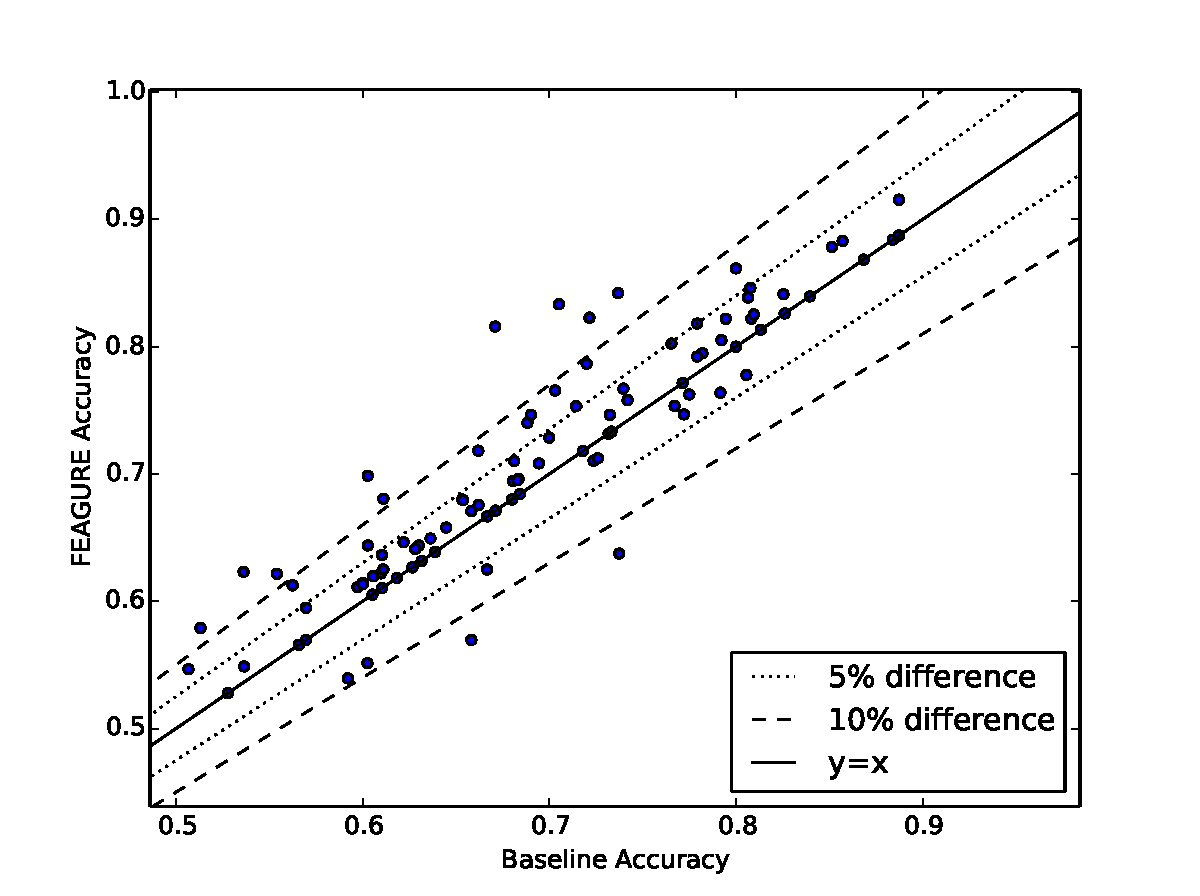
\includegraphics[width=0.8\linewidth]{new_svm_10_base_vs_lvl1}
	\caption{Accuracy of
		baseline approach compared to single activation of FEAGURE (SVM). Each point represents a dataset. The dotted lines represent a 5 and 10 percent difference in accuracy}
	\label{fig:svm_base_lvl1}
\end{figure}

The results show a general trend of improvement, with high ($> 5\%$) or very high ($>10\%$) improvement being common. We also see that for 24 datasets, no improvement is seen. Of these, 4 have no generated features, and 20 have few of them, and those have not contributed to the performance of the classifier. In a small subset of the datasets, we see a degrade in accuracy, with 4 of the 100 datasets showing a degrade of over $> 5\%$. 

In their paper on TechTC-100, \citeA{gabrilovich2004text} define a metric known as Maximal Achievable Accuracy (MAA). This criterion attempts to define the difficulty of the induction problem by finding the maximal accuracy among three induction algorithms (SVM, K-NN and CART \footnote{\citeA{breiman1984classification}}).
Intuitively, a dataset with low MAA can be considered harder than one with a high MAA, since a known induction algorithm can achieve a higher accuracy for it.
Figure \ref{fig:25best} shows the 25 hardest datasets in TechTC-100, in terms of the MAA criterion. 
We see that for 7 of these, there is no change in accuracy, either due to the lack of features or due to lack of contribution in the final classifier.
For 11 of the 25 datasets, we see a minor improvement in accuracy. For 6 of them, we see an improvement of $5\%$ or above, with the highest being over $20\%$.
Of the 25 datasets, only a single dataset shows a degrade in accuracy. This results illustrates that we can, in general, rely on FEAGURE to yield positive features for difficult classification problems.

\begin{figure}
	\centering
	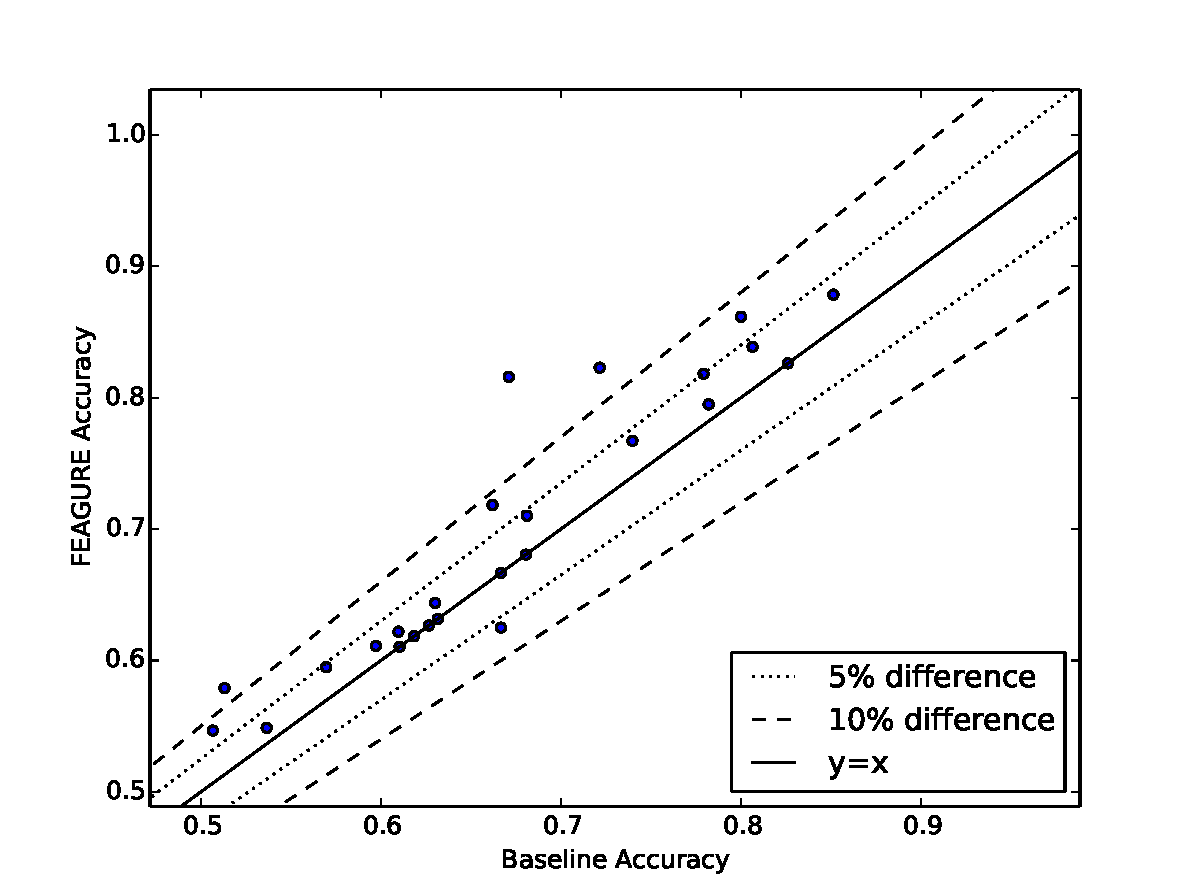
\includegraphics[width=0.8\linewidth]{new_svm_10_25hardest}
	\caption{Accuracy of
		baseline approach compared to single activation of FEAGURE (SVM). Displayed are the 25 hardest datasets (meaning they have the lowest MAA)}
	\label{fig:25best}
\end{figure}

\subsection{Using Non-Tree classifiers with FEAGURE}

As we have discussed in section \ref{algorithm_section}, algorithm \ref{code-creating-prob} creates a generic learning problem as part of its execution. In this section, we will test the effects of using various induction algorithms on these recursive problems. We have chosen to try both K-NN and SVM, with the following parameters: For K-NN, we used $K=3$. For SVM we used $C=10$, with both Linear and a Radial Basis Function (RBF) kernels.

%Table \ref{table:features-nontree} shows the average number of generated features. We see that these approaches generate far fewer features on average. This should come as no surprise, as we cannot flatten constructed recursive trees in order to generate additional features, nor do we run the learning algorithms on smaller problems.
Table \ref{table:acc-nontree} shows the accuracies achieved by using these induction algorithms. We see that while in general, the results are slightly poorer than those achieved by our approach, they are roughly comparable, and in some cases perform noticeably better. One particular such case is that of K-NN for the OHSUMED dataset, which was previously the only case where no improvement in accuracy was achieved. Using an SVM classifier to generate features rather than tree-based features, we see an improvement in accuracy for this case. This may be due to the nature of RBF-based classifiers, which look at distance between examples, similarly to K-NN.
Looking at the number of features generated, we see that on average, these approaches generate far fewer features. This should come as no surprise, as the tree-based classifier uses flattening to create additional features.

%\begin{table}[]
%	\centering
%	\caption{Average Number of Generated Features}
%	\label{table:features-nontree}
%	\begin{tabular}{lllll}
%		& \# Features(Tree)  & \# Features(Linear SVM)  & \# Features(RBF SVM) & \# Features(3-NN) \\
%		OHSUMED      & 506.2  &  24.7 & 34.5  & 14.6     \\
%		TechTC-100  & 63.3   &   12.04    &  8.95   & 4.25        
%	\end{tabular}
%\end{table}

\begin{table}[]
	\centering
	\caption{Average accuracy over all datasets. The columns specify the induction algorithm used in FEAGURE (Decision Tree, SVM with linear or RBF kernel, K-NN). The rows specify the induction algorithm used on the generated features for evaluation. TechTC-100 has an additional entry for 5\% feature selection, meaning only 5\% of all features are used.}
	\label{table:acc-nontree}
	\centering
	\begin{tabular}{|l | l || l | l| l|l|}
		\hline
		Dataset & Classifier  & Tree-FEAGURE & Linear SVM   & RBF SVM & 3-NN    \\ \hline
		\multirow{2}{*}{OHSUMED} & KNN  & 0.761 & 0.756   & \textbf{0.783} & 0.744 \\ \cline{2-6}
		& SVM   & \textbf{0.814}  & 0.795  & 0.796 & 0.788 \\ \specialrule{.15em}{.05em}{.01em} % \hline
		
		\multirow{2}{*}{TechTC-100} & KNN  & \textbf{0.533} & 0.531 ($p<0.05$) & 0.527 &  0.528 \\ \cline{2-6}
		& SVM    & \textbf{0.712} &  0.705 ($p<0.005$)  & 0.698 ($p<0.05$) & 0.697 \\ \specialrule{.15em}{.05em}{.01em}
		
		\multirow{2}{*}{TechTC-100 (5\%)} & KNN  & \textbf{0.629 ($p<0.001$)}  & 0.625 ($p<0.05$) & 0.61 & 0.617 \\ \cline{2-6}
		
		& SVM   & \textbf{0.707 ($p<.001$)} & 0.697 & 0.7 ($p<0.05$) & 0.699 ($p<0.05$)\\ \hline
		
	\end{tabular}
\end{table}

\subsection{The Effects of Feature Filtering on Accuracy}
\label{result-maximal-average}

In this section we look at the effect of using a different evaluation method for generated features. In algorithm \ref{code-tree-thing}, we use a comparison function which compares the constructed feature to the existing feature map. 
For the most part, we compared the IG Ratio of the constructed feature to the maximal IG Ratio of features in $F$ to do so.
An alternative method to this is to use the mean IG Ratio of features in $F$. Should our new feature score lower than the average, we filter it out. 

%\begin{table}[]
%	\centering
%	\caption{Average Number of Generated Features}
%	\label{table:features-average}
%	\begin{tabular}{lllll}
%		& FEAGURE  & FEAGURE 2-level  & Average IG &  Average IG 2-level \\
%		OHSUMED      & 506.2           & 732        &    1270.6   &   1371.4       \\
%		TechTC-100  & 63.3       & 65.06      &  234.43 &  244.05             
%	\end{tabular}
%\end{table}

\begin{table}[]
	\centering
	\caption{Average accuracy across all datasets. The columns specify feature filtering approach, being either the average information gain (IG) or the maximal. The rows specify the induction algorithm used on the generated features for evaluation. TechTC-100 has an additional entry for 5\% feature selection, meaning only 5\% of all features are used.}
	\label{table:acc-average}
	\begin{tabular}{|l | l || l | l || l| l|}
		\hline
		Dataset & Classifier & Max-IG   & Average-IG & Max-IG 2-level  & Average-IG 2-level    \\ \hline
		\multirow{2}{*}{OHSUMED} & KNN  & \textbf{0.761} & 0.667 & 0.744   & 0.686 \\ \cline{2-6}
		& SVM  & \textbf{0.814} & 0.811   & 0.808    & 0.81 \\ \specialrule{.15em}{.05em}{.01em} % \hline
		
		\multirow{2}{*}{TechTC-100} & KNN & 0.533 & 0.553 ($p<0.001$) & 0.552 & \textbf{0.555 ($p<.001$)}  \\ \cline{2-6}
		& SVM  & 0.712 & \textbf{0.728 ($p<0.001$)}    & 0.691   & 0.653 \\ \specialrule{.15em}{.05em}{.01em}
		
		\multirow{2}{*}{TechTC-100 (5\%)} & KNN  & 0.629 & \textbf{0.646 ($p<0.001$)} & 0.619   & 0.594 \\ \cline{2-6}
		
		& SVM  & 0.707 & \textbf{0.724 ($p<.001$)}   &0.704 & 0.707 ($p<0.05$) \\ \hline
		
	\end{tabular}
\end{table}

%Table \ref{table:features-average} shows the amount of features generated by FEAGURE. We see that the amount is significantly greater, indicating that this is a more lax requirement than the one we used (over half of the best information gain ratio). 
Table \ref{table:acc-average} shows the accuracies attained through this change. For the TechTC-100 dataset collection, we see a noticeable increase in accuracy, especially for single level application. For the OHSUMED dataset, however, we cannot detect a meaningful improvement, and for K-NN see a significant degrade in accuracy. 
Looking at he number of features generated reveals that using the average IG method for filtering yields roughly three times as many features for TechTC-100 (compared to using maximal IG ratio). For the OHSUMED dataset, the number of features generated is roughly twice as much as that seen when using maximal IG, and that number is already quite high. 
These results suggest that for small problems, generating additional features may be preferable, whereas for ones with many examples, a stronger filtering mechanism is more advantageous. 


\subsection{The Effect of Search Tree Depth on Accuracy}

In this section, we test at the usefulness of searching local problems for additional features.
To do so, we ran FEAGURE while limiting the depth of the search tree in algorithm \ref{code-tree-thing}. 
We compare our two datasets side-by-side.

\begin{figure}
	\centering
	\begin{subfigure}{.55\textwidth}
		\centering
		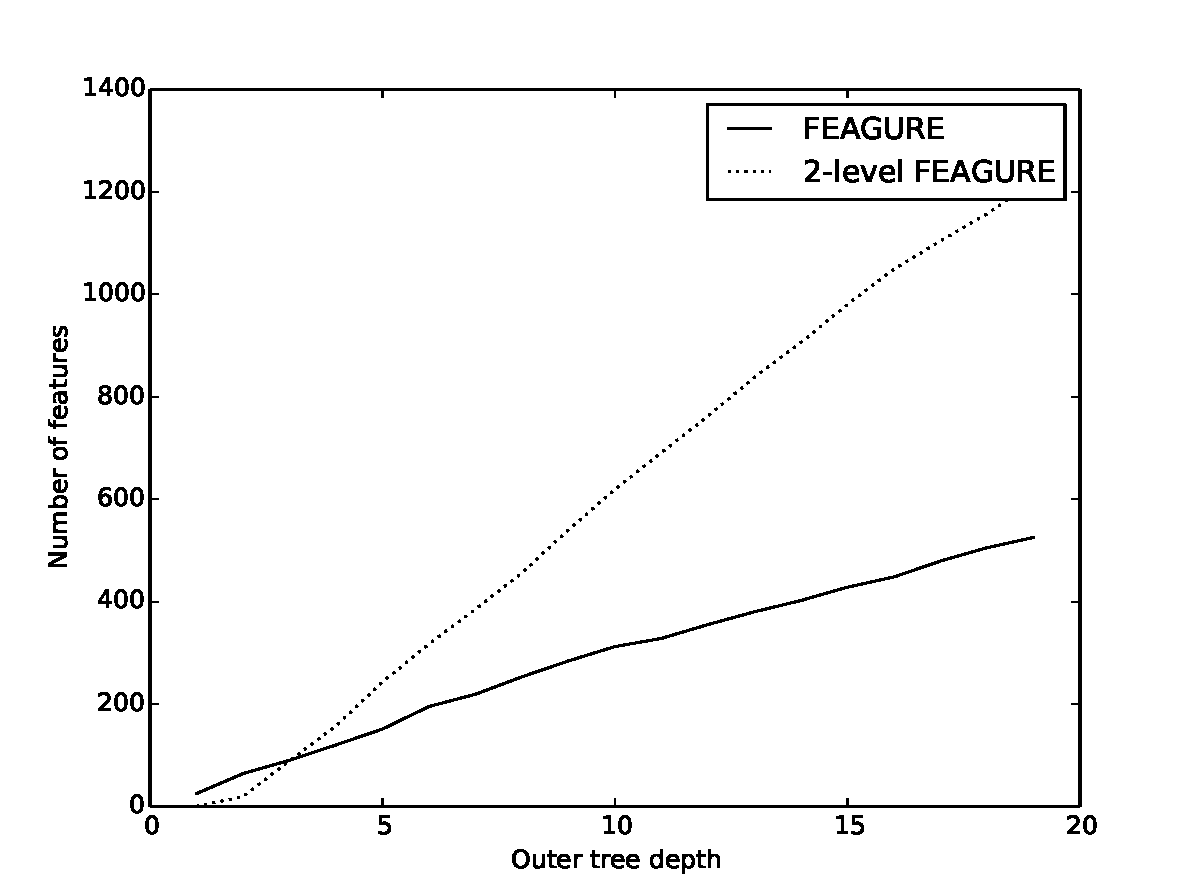
\includegraphics[width=1.1\linewidth]{num_features_ohsumed.pdf}
		\caption{OHSUMED}
		\label{fig:features-depth-ohsumed}
	\end{subfigure}%
	\begin{subfigure}{.55\textwidth}
		\centering
		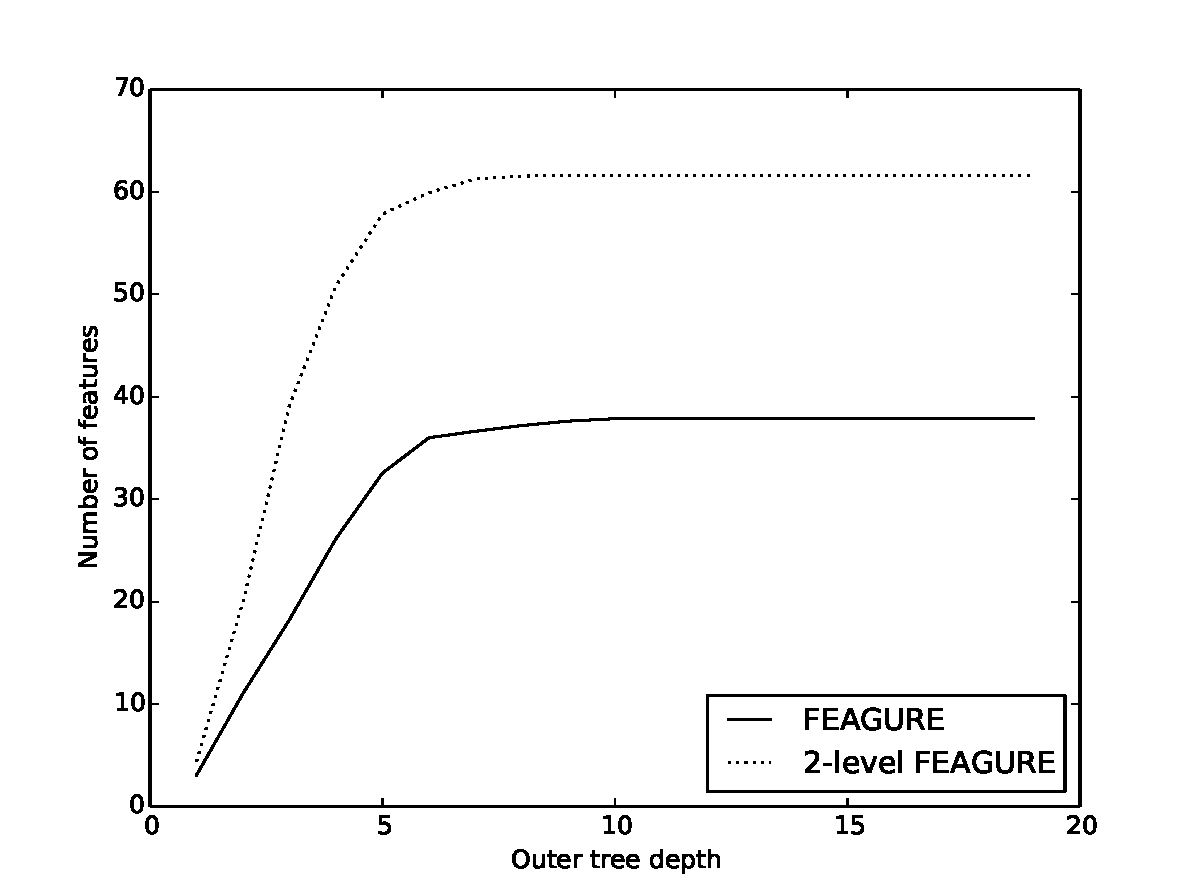
\includegraphics[width=1.1\linewidth]{num_features_techtc.pdf}
		\caption{TechTC-100}
		\label{fig:features-depth-techtc}
	\end{subfigure}
	\caption{Mean number of features generated}
	\label{fig:features-depth}
\end{figure}

Figure \ref{fig:features-depth} shows the number of generated features per maximal depth.  For both datasets, we see a linear increase, with a two-level application showing a faster increase. In TechTC-100, we see that after a certain depth, there is no additional gain. Due to the small size of the learning problems, beyond that depth the remaining training sets are too small to continue feature generation without significant risk of over-fitting, and thus FEAGURE stops its execution.

\begin{figure}
	\centering
	\begin{subfigure}{.55\textwidth}
		\centering
		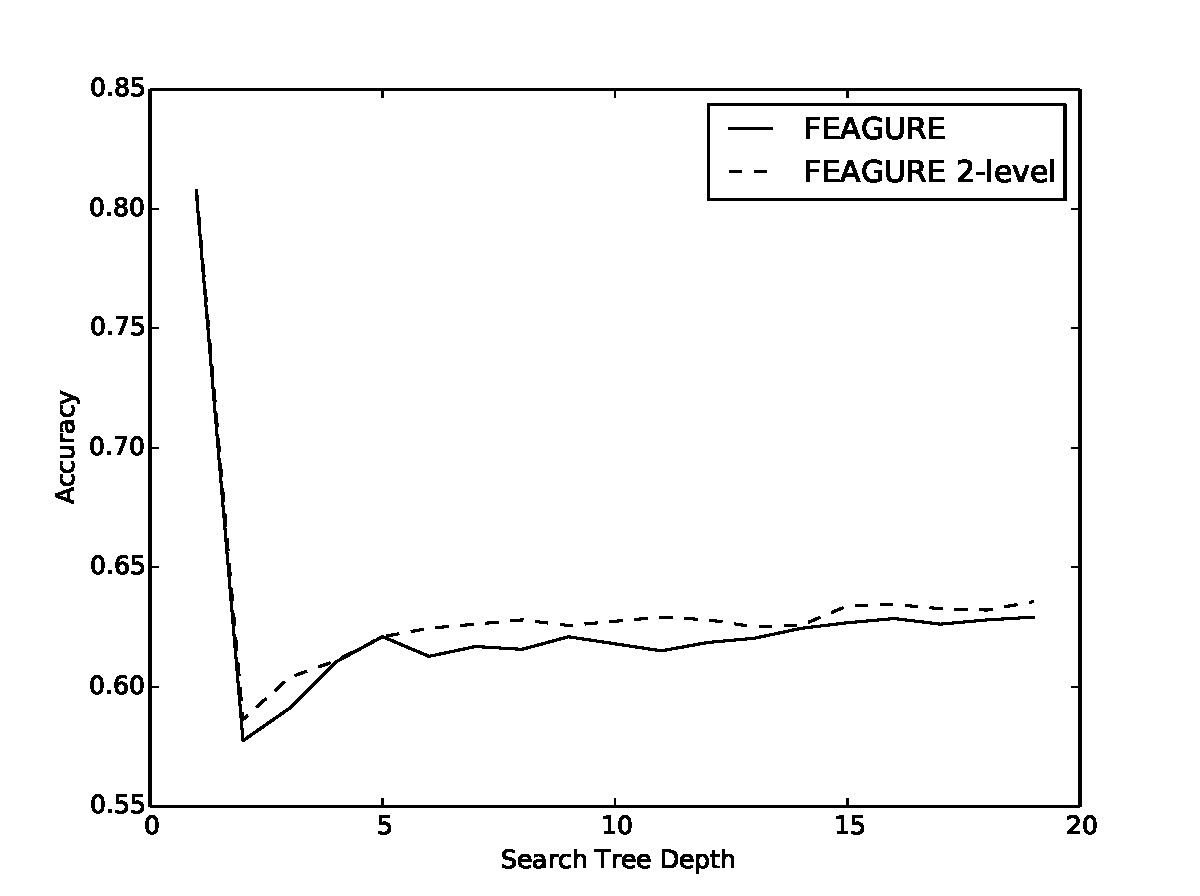
\includegraphics[width=1.1\linewidth]{new_depth_ohsumed.pdf}
		\caption{OHSUMED}
		\label{fig:svm-ohsumed}
	\end{subfigure}%
	\begin{subfigure}{.55\textwidth}
		\centering
		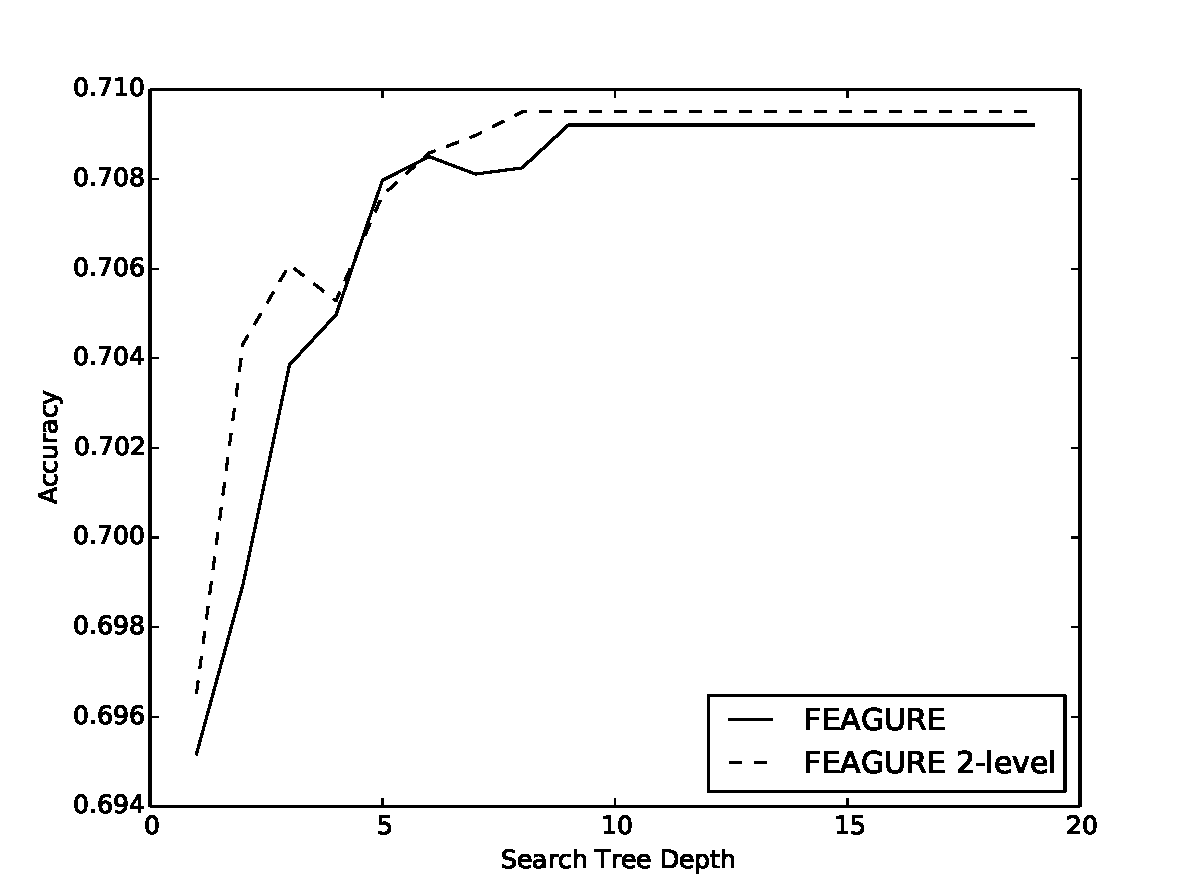
\includegraphics[width=1.1\linewidth]{new_depth_005_techtc.pdf}
		\caption{TechTC-100, with feature selection}
		\label{fig:svm-techtc}
	\end{subfigure}
	\caption{Mean SVM Accuracy across all datasets}
	\label{fig:svm-acc}
\end{figure}

Figure \ref{fig:svm-acc} shows the mean accuracy of a SVM classifier for increasing depths. The results for K-NN classifiers are similar in their general trend. For TechTC-100, we see a trend of increasing accuracy, up to a saturation point. This is to be expected, as adding largely orthogonal features would yield improvement until a maximal depth is achieved and no additional features are generated.

For OHSUMED, however, we see a sharp fall in accuracy, followed by a slow recovery. 
This effect can be attributed to the amount of features generated. As we have seen when looking at the average IG compared to the maximal in section \ref{result-maximal-average}, more features do not equate better accuracy. As we increase the search depth, however, the local nature of the problems alongside the orthogonality of new features allows us to locate a sufficient number of good features to improve accuracy once more.

In both cases, we see that the two level application of Deep-FEAGURE yields slightly better accuracy on average.

%\subsection{Qualitative Analysis}
%In order to better understand the contribution of these features, let us look at several of them to try and better understand them. Figure \ref{fig:level1_good} shows one of the features generated for single level feature generation. We can see that the feature attempts to separate based on geographical location. Figure \ref{fig:level1_simple} shows a simple feature regarding people, and showcases the fact that when there is no need for overly complex features, our technique will not force such features. This feature yields a $10\%-15\%$ increase in accuracy (depending on feature selection level), and is generated by both the single and two level approaches.

%Figure \ref{fig:level2_tree} showcases the additional power of the level two approach. The second level learning problem separates non-countries from countries, as well as countries which deal with non fuel manufacturing Arabic nations from those who embargo them.

%Figure \ref{fig:weird_trees} showcases some of the unique oddities of using our technique with the YAGO2 knowledge base. Since YAGO groups together all entities which have a grammatical gender (including fictional characters and non-living objects) under a single relation, the constructed feature looks at both deceased individuals and words that are the same as Australian television channels (such as Gold and Galaxy) at the same time.

%\begin{figure}[]
%	\centering
%	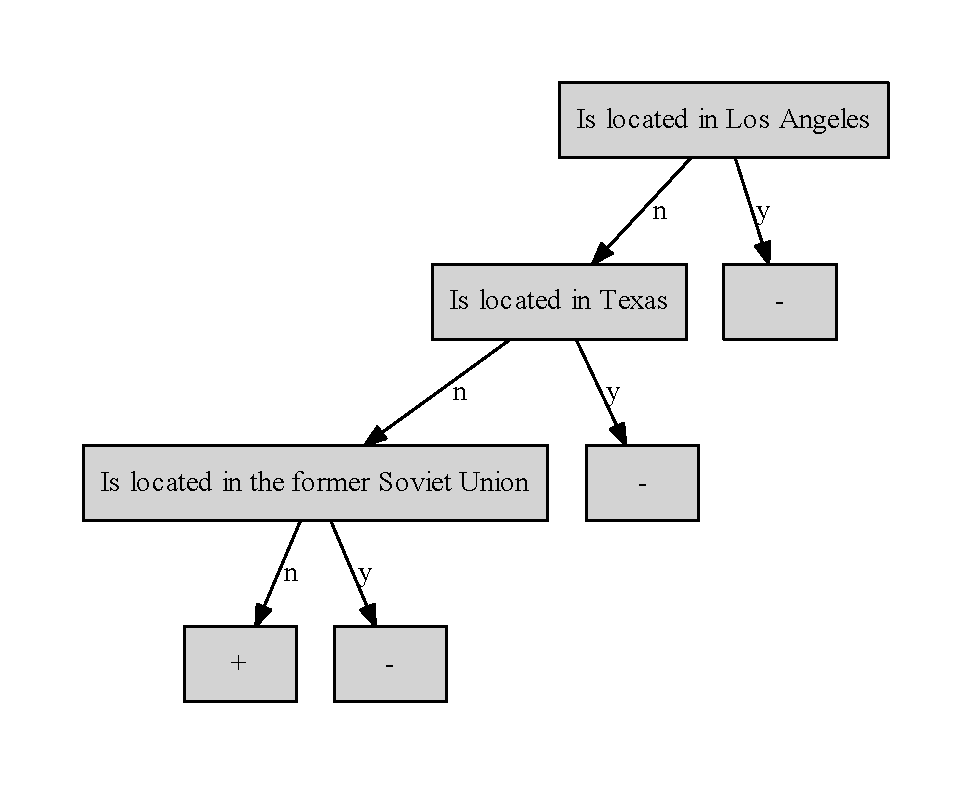
\includegraphics[width=0.8 \linewidth]{level1_good.pdf}
%	\caption{A single level feature regarding nations and organizations with official websites}
%	\label{fig:level1_good}
%\end{figure}

%\begin{figure}[]
%	\centering
%	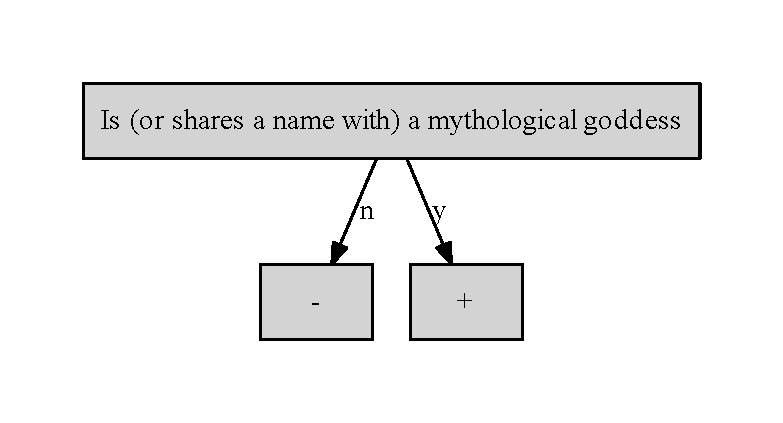
\includegraphics[width=0.6 \linewidth]{level1_simple.pdf}
%	\caption{A single level feature regarding people (real or fictional)}
%	\label{fig:level1_simple}
%\end{figure}

%\begin{figure}[]
%	\centering
%	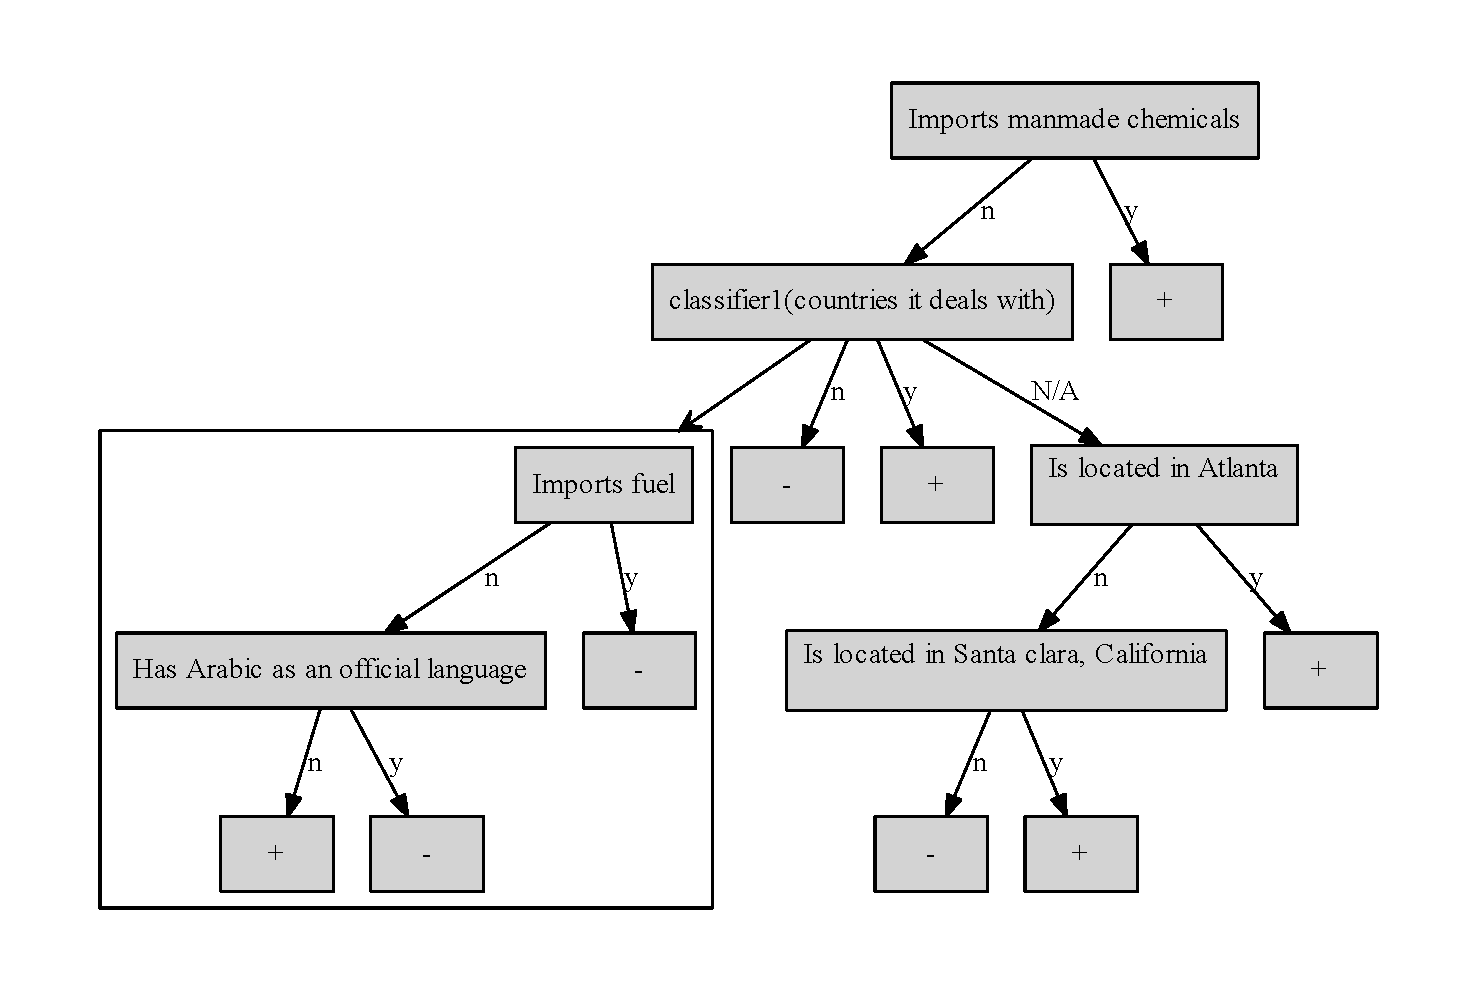
\includegraphics[width=\linewidth]{level2_tree.pdf}
%	\caption{A two level feature regarding countries and organizations}
%	\label{fig:level2_tree}
%\end{figure}

%\begin{figure}[]
%	\centering
%	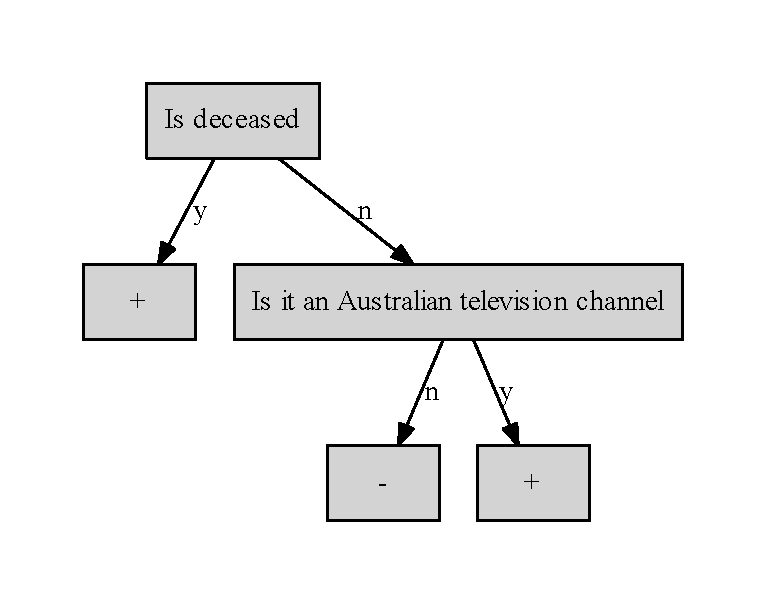
\includegraphics[width=0.6 \linewidth]{weird_trees.pdf}
%	\caption{A single level feature regarding things with a grammatical gender}
%	\label{fig:weird_trees}
%\end{figure}


\section{Related Work}

Feature generation approaches were found useful for a wide variety of learning problems \cite{markovitch2002feature,ragavan1993complex,utgo1991linear}.
These feature generation approaches search for new features that better represent the target concept than existing features. To that end, there are two major approaches for feature generation: combinational and using additional knowledge.
Combinational feature generation techniques aim to locate more descriptive features by combining existing features in various ways. The LDMT algorithm \cite{utgo1991linear}, for example, uses linear combinations of the original features to construct more informative ones. Another major class of combinational feature generation approaches is that of \emph{Deep Learning} \cite{lecun1998gradient,bengio2009learning,plotz2011featurefull,kim2013deepfull}. Deep learning techniques seek to create features through complex, non-linear combinations of existing features, allowing for a wide variety of possible features.

In contrast to combinational approaches, some feature generation algorithms, including FEAGURE, seek to inject additional knowledge into the existing learning problem. These approaches seek to do so almost exclusively through the use of relational data. 
Within this wide family of knowledge-based approaches, we can see a distinction between unsupervised, supervised and mixed approaches.
Unsupervised knowledge-based feature generation techniques aim to incorporate additional knowledge from external sources without consideration to the labels supplied by a given training set. They do so in several differing ways:
\begin{itemize}
	\item Concept based approaches such as ESA \cite{gabrilovich2009wikipediafull} ,for example, present a method for generating features that are based on semantic concepts. These approaches rely on complex techniques to create a mapping between existing data and the semantic concepts which serve as external knowledge.
	\item Propositionalization \cite{kramer2000bottom} approaches are a class of feature generation algorithms that rely on relational data to serve as external knowledge. They operate by using a combination of operators in order to create first-order logic predicates connecting existing data and relational knowledge.
	\citeA{cheng2011automatedfull} devise a generic framework to do so using linked data, and offer some insights into taxonomy-based features.
	The \emph{Shallow} algorithm described in section \ref{shallow_section} is a propositionalization algorithm.
	\item Data mining approaches such as FeGeLOD \cite{paulheim2012unsupervisedfull} aim to directly utilize linked data in order to automatically enrich existing data and make it more expressive.
\end{itemize}
These knowledge-based techniques serve as a powerful tool for feature generation based on knowledge. Despite this fact, the unsupervised nature of these approaches tends to lead to a shallow exploration of the knowledge base, as deep unguided search is computationally expensive, and leads to a potentially large number of features.

Unlike unsupervised approaches, some methods, FEAGURE included, seek to utilize a labelled training set in order to perform a more guided search. 
These techniques can trace their source to \emph{Inductive Logic Programming(ILP)} \cite{quinlan1990learning,muggleton1991inductive}, a supervised approach that induces a set of first-order formulae that define a good separation of the given training set.
 \emph{Upgrade} methods such as ICL \cite{van2001upgrade} and SGLR \cite{popescul200716} can be seen as the supervised equivalent of propositionalization methods. Instead of creating predicates a-priori, feature generation is performed during the training phase, in a more structured manner, allowing for complex features to be considered.
 While upgrade approaches bear some similarities to our approach, there are several critical differences, the key of which being the ability to more easily locate complex features through the use of existing induction algorithms. 

Another type of supervised, knowledge-based, feature generation approach is \emph{Relational Learning} techniques. These techniques are designed to utilize relational databases and expand their knowledge. One such technique is that of View Learning \cite{davis2005view}. View learning generates new relational tables from the existing relational knowledge, based on labelled data.
This approach bears similarity to our approach in that it can effectively utilize background knowledge to draw conclusions using the combination of labelled data and background knowledge. Unlike our approach, these views can be seen as binary rules, and require specific induction methods to be used.

FEAGURE itself is a supervised knowledge-based feature generation approach. It focuses on creation of recursive induction problems, in a manner reminiscent of view learning. Unlike view learning, the recursive construction of induction problems allows for complex exploration of features, which can then be combined in a more general way through the use of existing induction algorithms.
%can maybe elaborate more? talk about graph learning?

%works on linked data ? so can talk about uses in search / graph based algorithms / trying to do entity linking and then use it->us

%TODO:talk about entity linking? talk about linked data?

%Following this work, Relational Learning - techniques designed to utilize relational databases, have become increasingly prevalent. One such technique is that of View Learning \cite{davis2005view}, which generated new tables from existing ones, effectively performing feature generation for relational methods.
%Unlike View Learning and other Relational Learning methods, our approach constructs a new learning problem in a different domain using the existing problem as a guide. Essentially,  we try to re-think our problem from a new direction, rather than trying to fit increasingly less connected entities to the original problem. Furthermore, the ability of our approach to locate locally beneficial features which may be difficult to otherwise detect is invaluable. Finally, we note that the use of decision trees during the feature generation process allows for a natural method by which to filter out features even before applying traditional feature selection mechanisms.

\section{Conclusions}
%finishing up and summary

In this paper, we proposed FEAGURE, a supervised feature generation algorithm for using knowledge bases. Our approach is based around the concept of injecting traditional induction algorithms with external knowledge through the use of features constructed in a supervised manner based on the target concept. 

In section \ref{formal}, we 
%talk about induction vs deduction?

%talk about the algorithm's main ideas through the use of the example?

%talk about evaluating our algorithm on text categorization, and finding it good

%talk about potential strengths and weaknesses (can do complex+efficient search/tradeoff by limiting search and generation. use of local problems may cause overfitting)
%like any algorithm based on this data, dependent on good, strong entity linking of the values to the knowledge base(vs combination approaches which don't)

%anything else?

%We presented a novel new approach to feature generation using relational data, based on constructing and solving new learning problems in the relational domain. 
%Our feature generation algorithm constructs powerful and complex features, and can identify locally useful features as well as general trends. These features can be used along any traditional machine learning algorithm.
%While we focused on applying this approach to text categorization problems, it is important to note that it is applicable to any classification problem where feature values are categorical and have semantic meanings, such as drug names, cities and so on. Although there is no simple way to generalize this approach to numeric features, we believe there are numerous domains where feature values do have semantic meaning, even excluding text-based domains.
%While our approach only generates binary features, aggregation based techniques such as those used in SGLR apply here as well. We furthermore note that when solving non-binary classification problems, we can construct categorical features with, at most, the same amount of values as there are labels in the dataset.

%A major source for potential improvement is the subject of matching values to semantic objects. Given the major advances in the field of Wikification \cite{bunescu2006using} in general and Entity Linking \cite{rao2013entity} in particular, these approaches can be used to link the initial text to entities within the semantic data without losing information, which may lead to better results, especially for text classification problems. We have seen in our experiments that primitive entity matching techniques may lead to mistakes which can cascade into poor features.

%Another major potential avenue for improvement is to use the labelling techniques discussed section \ref{algorithm_section} as a way to directly label entities within the semantic graph, which yields a Collective Classification \cite{kajdanowicz2013collective} problem in the semantic domain. Solving this learning problem in turn allows us to label any entity within the semantic net, essentially yielding a labelled semantic net trained on our problem. We can then use this net to label new objects within the original problem context through a combination of entity extraction, usage of the semantic labels and label consolidation techniques.

\clearpage
\vskip 0.2in
\bibliographystyle{theapa}
\bibliography{document}
%\bibliographystyle{plainnat}
%\bibliography{document}

\end{document} 